%!TEX TS-program = pdflatex
\documentclass[runningheads,envcountsame]{llncs}
%
\usepackage[T1]{fontenc}
% T1 fonts will be used to generate the final print and online PDFs,
% so please use T1 fonts in your manuscript whenever possible.
% Other font encondings may result in incorrect characters.
%
\usepackage{graphicx}
\usepackage{tikz}

\usepackage{amsmath}
\usepackage{amssymb}

\usepackage{verbatim}
\usepackage[linesnumbered]{algorithm2e}

\spnewtheorem{claim*}[lemma]{Claim}{\itshape}{\normalfont}
\spnewtheorem*{cproof}{Proof of Claim}{\itshape}{\rmfamily}

\newenvironment{claimproof}
{\begin{cproof}
}
{\hfill$\blacksquare$
\end{cproof}
}

\spnewtheorem{thm}{Theorem}{\bfseries}{\itshape}

\newenvironment{proof*}
{\begin{proof}
	}
	{\qed
\end{proof}}

\newcommand{\angl}[1]{\langle #1 \rangle}
\newcommand{\dom}[1]{\text{dom}(#1)}
\newcommand{\sem}[1]{\text{range}(#1)}
\newcommand{\ren}{\bigsqcup}
\newcommand{\rk}{\text{rk}}
\def \<#1>{{\langle {#1} \rangle}}
\newcommand\lcop[1]{\left\lfloor{#1}\right\rfloor}
\newcommand\paras[1]{\mathsf{ps}(#1)}
\newcommand\he[1]{\mathsf{ht}(#1)}
\newcommand\comp[1]{\mathsf{comp}(#1)}
\newcommand\nop{\$}
\newcommand\pout{\mathit{pOut}}
\newcommand\tree[1]{\mathcal{T}_{#1}}
\newcommand\emp{\emptyset}
\newcommand\eps{\varepsilon}
\newcommand\ab{\allowbreak}
\newcommand\rhs{\mathit{rhs}}
\newcommand\ot{\leftarrow}
\newcommand\sos[1]{[\![#1]\!]}

\newcommand{\N}{\mathbb{N}}
\newcommand\SC{\mathfrak{S\!C}}
\newcommand\MTTR{\text{MTT}^\text{R}}

\begin{document}
\title{Deciding Linear Height and Linear Size-to-Height Increase of
  Macro Tree Transducers}
%TODO Please add
%
\titlerunning{Deciding Linear Increase Properties of Macro Tree Transducers}
% If the paper title is too long for the running head, you can set
% an abbreviated paper title here
%
\author{Paul Gallot\inst{1}\and
        Sebastian Maneth\inst{1} \and
        Keisuke Nakano\inst{2} \and
        Charles Peyrat\inst{3}
}
%
\authorrunning{P. Gallot, S. Maneth, K. Nakano, and C. Peyrat}
% First names are abbreviated in the running head.
% If there are more than two authors, 'et al.' is used.
%
\institute{Universit\"at Bremen, Germany \and
  Tohoku University, Sendai, Japan\and
  ENS Paris-Saclay, France
}

\maketitle

%TODO mandatory: add short abstract of the document
\begin{abstract}
We present a novel normal form for (total deterministic) macro tree transducers (mtts),
called ``depth proper normal form''. If an mtt is in this normal form,
then it is guaranteed that each parameter of each state of the mtt appears 
at arbitrary depth in the output trees of that state. Intuitively, if some parameter
only appears at certain bounded depths in the output trees of a state, then
this parameter can be removed by in-lining the corresponding output paths at
each call site of that state. We use regular look-ahead in order to determine
which of the paths should be in-lined. As a consequence of changing the look-ahead,
a parameter that was previously appearing at unbounded depths,
may be appearing at bounded depths for some new look-ahead; for this reason, our
construction has be iterated in order to obtain an mtt in depth-normal form.
Using the normal form, we can decide whether the translation of an mtt
has linear height increase or has linear size-to-height increase.
\end{abstract}

\section{Introduction}
Current quantum hardware is unable to carry out universal quantum computations due to the buildup of errors that occur during the computation. 
The magnitude of the individual error is currently above the value that the Threshold Theorem requires in order to kick-start quantum error correction and fault-tolerant quantum computation~\cite[Section 10.6]{nielsen_chuang_2010}. 
Although the experimentally achieved fidelity rates are promising and the error bounds are inching closer to the required threshold, we will have to work for the foreseeable future with quantum hardware with errors that build-up during the computation.  This implies that we can only do a limited number of steps before the output of the computation has become completely uncorrelated with the intended one.

For fault-tolerant quantum computing, we repeat four steps: 
1) We apply a number of single and two-qubit quantum gates, in parallel whenever possible; 
2) We perform a syndrome measurement on a subset of the qubits; 
3) We perform fast classical computations to determine which errors have occurred and how to correct them; 
and, 4) We apply correction terms based on the classical computations.
We then repeat these four steps with a next sequence of gates. 
These four steps are essential to fault-tolerant quantum computing. 


The starting point of this work is to use the four steps outlined above, not to carry out error correction and fault-tolerant computation, but to enhance short, constant-depth, {\em uncorrected} quantum circuits that perform single qubit gates and {\em nearest-neighbor} two qubit gates. 
Since in the long run we will have to implement error-correction and fault-tolerant computation anyhow, and this is done by such a four-step process, why not make other use of this architecture? Moreover, on some of the quantum hardware platforms, these operations are already in place.
Embracing this idea we naturally arrive at the question: what is the computational power of \textit{low-depth} quantum-classical circuits organized as in the four steps outlined above? 
We thus investigate circuits that execute a small, ideally constant, number of stages, where at each stage we may apply, in parallel, single qubit gates and {\em nearest-neighbor} two qubit gates, followed by measurements, followed by low-depth classical computations of which the outcome can control quantum gates in later stages. 
It is not clear, at first, whether such circuits, especially with constant depth, can do anything remotely useful. 
But we will see that this is indeed the case: many quantum computations can be done by such circuits in constant depth. 
By parallelizing quantum computations in this way, we improve the overall computational capabilities of these circuits, as we do not incur errors on qubits that are idle, simply because qubits are not idle for a very long time. 
Furthermore, reducing the depth of quantum circuits, at the cost of increasing width, allows the circuit to be run faster even if errors occur.

The first usage of such a four-step layout, not to do error correction, but to perform computations, can be found in the paradigm of measurement-based quantum computing~\cite{gottesman1999demonstrating,raussendorf2001one,jozsa2006introduction,clark2007generalised}: 
A universal form of quantum computing where a quantum state is prepared and operations are performed by measuring qubits in different bases, depending on previous measurements and intermediate measurements.

\citeauthor{PhamSvore2013} were the first to formalize the four-step protocol for performing computations~\cite{PhamSvore2013}. They included specific hardware topologies by considering two-dimensional graphs for imposing constraints on qubit interactions. In their model, they develop circuits for particularly useful multi-qubit gates, including specifying costs in the width, number of qubits, depth, number of concurrent time steps, size, and total number of non-Identity operations.
As a result, they find an algorithm that factors integers in polylogarithmic depth.
\citeauthor{Browne:2011} showed that the main tool in the work by \citeauthor{PhamSvore2013}, the fan-out gate, can also be replaced by additional log-depth classical computations in the measurement-based quantum computing setting~\cite{Browne:2011}.

More recently, \citeauthor{Cirac:2021} introduced a scheme to implement unitary operations involving quantum circuits combined with Local Operations and Classical Communication ($\mathsf{LOCC}$) channels: $\mathsf{LOCC}$-assisted quantum circuits~\cite{Cirac:2021}. Similarly to the four-step scheme we just described, they allow for a short depth circuit to be run on the qubits, followed by one round of $\mathsf{LOCC}$, in which ancilla qubits are measured and local unitaries are applied based on the measurement outcomes. They show that in this model any 1D transitionally invariant matrix-product state (MPS) with fixed bond dimension is in the same phase of matter as the trivial state. Similar ideas can be found in~\cite{TVV_NonAbelianTopologicalOrder_2022, tantivasadakarn2021long}.

In this work, we introduce a new model, called \textit{Local Alternating Quantum-Classical Computations} ($\LAQCC$). In this model we alternate between running quantum circuits (constrained by locality), ending in the measurement of a subset of qubits, and fast classical computations based on the measurement results. The outcome of the classical computations are then used to control future quantum circuits. We allow for flexibility in this model, by giving different constraints to the power of both the quantum circuits and the classical circuits as well as the number of alternations between them. 
Most attention will be given to $\LAQCC$ containing quantum circuits of constant depth, classical circuits of logarithmic depth and at most a constant number of alternations between them. 
Any circuit constructed in this model is considered to be of constant depth. 
We restrict ourselves to logarithmic depth classical computations, as this is the first natural and non-trivial extension beyond constant-depth classical computations. 
Constant-depth classical computations do however also have an equivalent constant-depth quantum implementation.

The definition of $\LAQCC$ sharpens the original definition of \citeauthor{PhamSvore2013} by adding constraints to the intermediate classical computations. This allows us to bound the power of $\LAQCC$ from above. 

The main result of \citeauthor{Cirac:2021}, that 1D translational invariant MPS with fixed bond dimension can be prepared by $\mathsf{LOCC}$-assisted circuits, relies on local symmetries of the MPS. These symmetries allow them to prepare local states (on a constant number of qubits) and glue them together by doing one round of the appropriate entangling measurement and corrections, after which they run a round of local unitaries to get the desired result. This general scheme for preparing states that exhibit an MPS description with the appropriate local symmetries requires only geometrically local unitaries and one round of measurement and corrections an therefore is accessible in $\LAQCC$. Studying different local symmetries, known as Symmetry Protected Topological (SPT) phases of matter, to find measurement-based constant depth circuits for states is a broad ongoing field of research~\cite{TVV_NonAbelianTopologicalOrder_2022, tantivasadakarn2021long, smith2023deterministic}. 
All these schemes have a $\LAQCC$ implementation.

%$\LAQCC$-circuits also exist for general schemes of preparing local states, based on the local tensors, and gluing them together using one round of entangled measurement and corrections, based on the local symmetry. 
%The main result of \citeauthor{Cirac:2021}, that 1D translational invariant MPS with fixed bond dimension can be prepared by $\mathsf{LOCC}$-assisted circuits, relies heavily on local symmetries of the MPS and as a result also has an equivalent $\LAQCC$ implementation. 
%The corrections applied after the measurement round are local unitaries depending on the local symmetries of the MPS. 

 

%This general scheme of preparing local states, based on the local tensors, and gluing it together by doing one round of entangled measurement and corrections, based on the local symmetry, is accessible in $\LAQCC$.
Note however that \citeauthor{Cirac:2021} also suggest a circuit for the $W$-state.
This circuit uses sequentially and dependent measurement-based corrections of the ancilla qubits. 
These dependent measurements translate to sequential alternations between the quantum and classical circuits and therefore increase the total depth to linear depth, exceeding the constant-depth constraints imposed by $\LAQCC$-circuits. 

We study the power of the $\LAQCC$ model with respect to state preparation, showing that even with only constant quantum-depth and logarithmic classical depth it remains possible to prepare states with long-range entanglement.
Another surprising result is that it is unlikely that $\LAQCC$ circuits are classically simulatable. We show that any instantaneous quantum polynomial-time (IQP) circuit~\cite{Bremner2010,Shepherd2009} has an $\LAQCC$ implementation.
Classical simulation of IQP circuits implies the collapse of the polynomial hierarchy to the third level, which is not believed to be true~\cite{Bremner2017}. Therefore, we expect that $\LAQCC$ circuits are unlikely to be classically simulatable. We bound the power of $\LAQCC$ by showing that it is contained in $\QNC^1$, the class of polynomial-size, log-depth circuits.

Next, we also study the power that intermediate classical calculations can add to quantum computations, by considering a new model that alternates between polynomially many polynomial-depth quantum circuits and unbounded classical computations
We study this model by doing a complexity theoretical analysis, where we draw inspiration from the notions of complexity given by \citeauthor{RosenthalYuen:2022}, \citeauthor{MetgerYuen:2023}, and \citeauthor{Aaronson:2004}.
All three complexity notions are based on the notion of state preparation, instead of more traditional definition of complexity such as the decidability of a computational problem. 
The first two consider classes based on sequences of quantum states preparable by a polynomial-sized quantum circuit, where the circuits are uniformly generated by a computational class, for instance, the class $\mathsf{PSPACE}$, which results in the complexity class $\mathsf{StatePSPACE}$~\cite{RosenthalYuen:2022,MetgerYuen:2023}.
The third notion considers a relative complexity, where the complexity is measured between two given states, and is measured by the number of gates, from a given gate-set, required to transform one state in another state~\cite{Aaronson:2004}. 
For our definition of state preparation complexity, we drop the uniformity constraint from~\cite{RosenthalYuen:2022,MetgerYuen:2023} and define a class as $\mathsf{StateX}$, which refers to states preparable by circuits of type $\mathsf{X}$. 
As an example, if $\mathsf{X} = \QNC^0$, this results in the class $\mathsf{StateQNC^0}$, which is the set of states preparable from the $\ket{0}^n$ state by poly-size constant-depth circuits. 
This notion is similar to the relative complexity from~\cite{Aaronson:2004}, where one state is the  $\ket{0}^n$ state and instead of counting the number of gates we consider the set of states preparable by a fixed number of gates. Using this notion of complexity we show that any state preparable by an $\LAQCC^*$ circuit is also preparable by a $\mathsf{PostQPoly}$ circuit, the class of circuits of polynomial depth with an additional post-selection gate. 

All Clifford circuits have a constant-depth $\LAQCC$ implementation, implying that any stabilizer state can be implemented by a constant-depth $\LAQCC$ circuit, see Section~\ref{sec:clifford_circuits} for a proof of this statement. 
Efficient circuits for stabilizer states have been known already through measurement-based quantum computing. Therefore this paper focuses on the preparation of non-stabilizer states, and as a surprising result we find novel constant-depth protocols for four very natural classes of non-stabilizer states.
Despite the extensive research into these four classes of non-stabilizer states and the many applications of them, no efficient constant- or low-depth state preparation protocols are known yet. We specifically consider these four classes as they are all often used as initial states in other algorithms.

The first state is a uniform superposition over an arbitrary number of states. 
This state finds applications in many quantum algorithms, as they often start with a uniform superposition over multiple states. 
This superposition is often achieved by applying Hadamard gates to every qubit due to its simplicity to prepare. 
Yet, the analysis of many algorithms, such as Shor's algorithm~\cite{Shor:1997}, would benefit from a different initial superposition. 
The circuit to prepare the uniform superposition over an arbitrary number of states uses an exact version of Grover search as a subroutine, that turns a probabilistic circuit, with a known constant probability of success, into a deterministic circuit. 
We use the circuit for preparing a uniform superposition over an arbitrary number of states as a subroutine in the next two quantum state preparation protocols. 

The second state is the $W$-state, the uniform superposition over all computational basis states of Hamming-weight~$1$, a natural long-ranged entangled state that displays a fundamentally nonequivalent type of entanglement from the Greenberger–Horne–Zeilinger state~\cite{WState:2000}, for which $\LAQCC$-type constant-depth circuits were previously known~\cite{PhamSvore2013, Cirac:2021}. 
The $W$-state is often used as benchmark for new quantum hardware~\cite{Haffner2005,Neeley2010,GarciaPerez:2021}. 
A novel way to prepare the $W$-state therefore gives a new way to benchmark different quantum devices with each other. 
A circuit for preparing the $W$-state was given in~\cite{Cirac:2021}, but this implementation requires sequentially alternating measurements followed by local unitaries, which in the $\LAQCC$ model is not considered to be of constant depth. 
We improve this protocol by giving an $\LAQCC$ implementation of the $W$-state, based on a compress-uncompress method that links the one-hot and binary encoding of integers.

The third state considered is the Dicke state, a generalization of the $W$-state, a superposition over all computational basis states with Hamming-weight $k$~\cite{Dicke:1954}. 
Dicke states have relevance in various practical settings.
For instance, for quantum game theory~\cite{zdemir2007}, quantum storage~\cite{Bacon_Compress:2006,Plesch:2010}, quantum error correction~\cite{ouyang2014permutation}, quantum metrology~\cite{toth2012multipartite}, and quantum networking~\cite{prevedel2009experimental}. 
Dicke states have been used as a starting state for variational optimization algorithms, most notably Quantum Alternating Operator Ansatz (QAOA)~\cite{Hadfield2019}, to find solutions to problems such as Maximum k-vertex Cover~\cite{Brandhofer2022,cook2020quantum}.
The ground states of physical Hamiltonians describing one-dimensional chains tend to show a resemblance to Dicke states such as states resulting from the Bethe ansatz, making them an ideal starting state when investigating the ground state behavior of these Hamiltonians~\cite{TDL_BetheAnsatzDerivation:2010,B_ExcitedStateQuantumPhaseTransitions:2013,DickeTransitions:2021}. 
For instance, the algorithm by \citeauthor{van2021preparing}, who give an algorithm to prepare the Bethe ansatz eigenstates of the spin-1/2 XXZ spin chain, starts by first preparing a Dicke state~\cite{van2021preparing}. 
A Dicke-state preparation protocol based on the compress-uncompress methodology used in the $W$-state furthermore finds applications in entanglement distillation, where the entanglement of a large state is concentrated on only a few qubits. 
Efficient deterministic circuits for preparing Dicke states have been proposed by \citeauthor{bartschi2019deterministic}~\cite{bartschi2019deterministic, bartschi2022deterministic_short_depth}. 
They provide a quantum circuit of depth $\mathO(k \log(\frac{n}{k}))$, allowing arbitrary connectivity, to prepare a Dicke state, which they conjecture to be optimal when $k$ is constant. 
In this work, we provide a constant-depth $\LAQCC$ circuit below their conjectured bound already for constant $k$. 
However, this does not directly disprove their conjecture, as we allow for intermediate measurements and classical computations. 
More significantly, we even construct constant-depth $\LAQCC$ circuits for $k = \mathO(\sqrt{n})$ greatly improving their bound.
This construction extends the compress-uncompress method for the $W$-state combined with additional subroutines. 

We continue with a log-depth state preparation protocol for the Dicke-state for arbitrary $k$. 
This protocol implements an efficient transformation between the factoradic number representation and the combinatorial number representation of a positive integer. 
The combinatorial number representation relates directly to the Dicke state. 
The provided efficient transformation between number representation systems might be of independent interest. 

We conclude by modifying our protocol for preparing a Dicke-state to a protocol that prepares quantum many-body scar states in constant-depth. 
These states have low entanglement and longer coherence times than states with similar energy density.
These characteristics make many-body scar states interesting to analyze and relevant within physics.
Many-body scar states appear for instance in the AKLT model~\cite{AKLT:1987,MRBAR:2018,MRB:2018} and different spin models~\cite{SI:2019,MOBFR:2020}.
Known methods for preparing these states have polynomial-depth~\cite{Gustafson:2023}, whereas our circuit has constant depth. 

% We conclude by studying the power that intermediate classical calculations can add to quantum computations. 
% In this study, we define a new model that relaxes constant-depth quantum circuits to polynomial depth quantum circuits, log-depth classical calculations to unbounded classical computations and a constant number of alternations to a polynomial number of alternations. 
% We call this model $\LAQCC^*$. 
% We study this model by doing a complexity theoretical analysis, where we draw inspiration from the notions of complexity given by \citeauthor{RosenthalYuen:2022}, \citeauthor{MetgerYuen:2023}, and \citeauthor{Aaronson:2004}.
% All three complexity notions are based on the notion of state preparation, instead of more traditional definition of complexity such as the decidability of a computational problem. 
% The first two consider classes based on sequences of quantum states preparable by a polynomial-sized quantum circuit, where the circuits are uniformly generated by a computational class, for instance, the class $\mathsf{PSPACE}$, which results in the complexity class $\mathsf{StatePSPACE}$~\cite{RosenthalYuen:2022,MetgerYuen:2023}.
% The third notion considers a relative complexity, where the complexity is measured between two given states, and is measured by the number of gates, from a given gate-set, required to transform one state in another state~\cite{Aaronson:2004}. 
% For our definition of state preparation complexity, we drop the uniformity constraint from~\cite{RosenthalYuen:2022,MetgerYuen:2023} and define a class as $\mathsf{StateX}$, which refers to states preparable by circuits of type $\mathsf{X}$. 
% As an example, if $\mathsf{X} = \QNC^0$, this results in the class $\mathsf{StateQNC^0}$, which is the set of states preparable from the $\ket{0}^n$ state by poly-size constant-depth circuits. 
% This notion is similar to the relative complexity from~\cite{Aaronson:2004}, where one state is the  $\ket{0}^n$ state and instead of counting the number of gates we consider the set of states preparable by a fixed number of gates. Using this notion of complexity we show that any state preparable by an $\LAQCC^*$ circuit is also preparable by a $\mathsf{PostQPoly}$ circuit, the class of circuits of polynomial depth with an additional post-selection gate. 

\paragraph{Summary of results}
\begin{itemize}
    \item We give a new definition of a computational model that captures the power of the four step process: applying a constant number of layers of one- and two-qubit gates; performing a syndrome measurement; perform a fast classical computation determining corrections; apply corrections. We call this model \emph{Local Alternating Quantum Classical Computations}, or $\LAQCC$ for short. In this model we bound the allowed quantum operations, intermediate classical calculations, and number of rounds separately. In Section~\ref{sec:LAQCC_model} we define this model and give a list of operations based on results from literature contained in this computational model. In some of these operations we explicitly use that we allow for multiple, but at most constant, rounds  of corrections.
    \item  We show show that there exist $\LAQCC$ circuits that can not be weakly simulated in Section~\ref{sec:IQP_in_LAQCC}. We further show that for every $\LAQCC$ circuit there exists a $\QNC^1$ circuit simulating it perfectly, in Section~\ref{sec:LAQCC_in_QNC1}.
    \item We introduce a new type computational complexity for preparing states and show that the extension of $\LAQCC$ where we allow a polynomial number of rounds and unbounded classical computation, is contained in $\mathsf{PostQPoly}$, the class of polynomial circuits with post-selection, in Section~\ref{sec:Complexity results}.
    \item We show a protocol to prepare the uniform superposition state of size $q$ in $\LAQCC$ using $\mathO(\ceil{\log_2(q)}^2)$ qubits in Section~\ref{sec:superposition_modulo_q}. 
    \item We show a protocol to prepare the $W_n$ state in $\LAQCC$ using $\mathO(n\log(n))$ qubits in Section~\ref{sec:W_state_in_LAQCC}.
    \item We show two ways of preparing the Dicke-$(n,k)$ state. The first method is in $\LAQCC$, works up to $k = \mathO(\sqrt{n})$, uses $\mathO(n^2\log(n))$ qubits, and is found in Section~\ref{sec:dicke:small_k}. The second method is in $\LAQCC\text{-}\mathsf{LOG}$ (an extension of $\LAQCC$ allowing for logarithmic number of alterations instead of constant), works for any $k$, uses $\mathO(\text{poly}(n))$ qubits, and is found in Section~\ref{sec:Dicke_in_LAQCC_LOG}. 
    \item We extend on our $\LAQCC$ method of generating Dicke-$(n,k)$ states for $k = \mathO(\sqrt{n})$ and show a protocol to generate many-body scar states for a particular Hamiltonian in $\LAQCC$ (Section~\ref{sec:many_body_scar}). 
\end{itemize}
Summarized in a table, we provide the following state generation protocols:
\begin{table}[htb]
\centering
\begin{tabular}{l|l|l|l}
\textbf{State description} & \textbf{Width} & \textbf{Depth} & \textbf{Implementation}\\
\hline 
Uniform superposition mod $q$: $\frac{1}{\sqrt{q}} \sum_{i = 0}^{q-1}\ket{i}$ & $\mathO(\ceil{\log^2 q})$ & $\mathO(1)$ & Section~\ref{sec:superposition_modulo_q}\\

$W$-state: $\frac{1}{\sqrt{n}}\sum_{i = 0}^{n-1}\ket{e_i}$ & $\mathO(n \log n)$ & $\mathO(1)$ & Section~\ref{sec:W_state_in_LAQCC}\\

Dicke-$(n,k)$, $k = \mathO(\sqrt{n})$: $\binom{n}{k}^{-1/2}\sum_{x \in \{0,1\}^n: |x| = k} \ket{x}$ &  $\mathO(n^2\log n)$ & $\mathO(1)$ 
&Section~\ref{sec:dicke:small_k}\\

Dicke-$(n,k)$: $\binom{n}{k}^{-1/2}\sum_{x \in \{0,1\}^n: |x| = k} \ket{x}$ & $\mathO(\text{poly}(n))$ & $\mathO(\log n)$ &Section~\ref{sec:Dicke_in_LAQCC_LOG}\\

QMBS: $\ket{S_k} = \frac{1}{k! \sqrt{\mathcal N(n,k)}}(Q^\dagger)^k \ket{\Omega}$ &  $\mathO(n^2\log n)$ & $\mathO(1)$  &  Section~\ref{sec:many_body_scar}
\end{tabular}
\caption{Summary of state preparation protocols given in this paper.}
\label{tab:sate_prep}
\end{table}
In the entry for the quantum many-body scar state $Q$ denotes the raising operator and $\mathcal N(n,k)=\binom{n-k-1}{k}$. 
Section~\ref{sec:many_body_scar} will provide more details on the variables and the implementation. 

\paragraph{Organization of the paper}
\noindent We first introduce relevant preliminaries in Section~\ref{sec:preliminaries}. 
In Section~\ref{sec:LAQCC_model} we formally define the class of Local Alternating Quantum-Classical Computations ($\LAQCC$). We also show that any Clifford circuit can be implemented in constant depth $\LAQCC$ (a result based on a result from measurement-based quantum computing~\cite{jozsa2006introduction}). 
This result allows us to give many useful multi-qubit gates and routines in Section~\ref{sec:gates_created_in_LAQCC}. 
Beyond that we show that constant depth $\LAQCC$ circuits are contained in $\QNC^1$ and that any $\mathsf{IQP}$ circuit has an $\LAQCC$ implementation.
We conclude this section with an analysis of a more powerful instantiation of $\LAQCC$ and show an inclusion with respect to the class $\mathsf{PostQPoly}$, which is the class of circuits of polynomial depth with one additional post-selection gate. 
In Section~\ref{sec:state_prep_in_LAQCC} we give $\LAQCC$ circuit implementations for preparing the uniform superposition over an arbitrary number of states, the $W$-state and the Dicke state up to $k = \mathO(\sqrt{n})$. We furthermore give a log-depth circuit implementation for preparing the Dicke state for any $k$. We conclude by showing a $\LAQCC$ circuit for generating many body scar states of a particular type of Hamiltonian.


\section{Preliminaries}
In this section, we describe the necessary background for automated planning and the significance of the International Planning Competition. 

% \subsection{Ontology}
% A formal ontology is typically represented as a set of concepts, relations, and axioms. A concept represents a set of objects or entities that share common properties, while a relation represents a connection or association between two or more concepts. Axioms are statements that define the relationships between concepts and relations. It is a formal representation of knowledge that is designed to facilitate automated reasoning and information processing. It acts as a structured vocabulary that describes a domain and promotes interoperability, data integration, and communication between humans and machines. Formally, an ontology $O$ can be represented as a tuple $(C, R, A)$, where $C$ is the set of concepts, $R$ is the set of relations, and $A$ is the set of axioms. Each concept \textit{c} $\in$ $C$ can be represented as a set of attributes, denoted as $Att(c)$. Similarly, each relation \textit{r} $\in$ $R$ can be represented as a set of attributes, denoted as $Att(r)$.

% Ontology is a branch of philosophy that deals with the nature of existence and being. In the field of computer science, however, ontology refers to a formal representation of knowledge that is designed to facilitate automated reasoning and information processing. It is a structured vocabulary that describes a domain and promotes interoperability, data integration, and communication between humans and machines. Various tools and methodologies, including Protege and ontology editors, are available for ontology creation. Ontologies are increasingly important in artificial intelligence, knowledge engineering, and the semantic web, and researchers are exploring their potential in diverse domains and applications.

% Figure environment removed

\subsection{Automated Planning}

Automated planning, also known as AI planning, is the process of finding a sequence of actions that will transform an initial state of the world into a desired goal state \cite{ghallab2004automated}. It involves constructing a plan or a sequence of actions that will achieve a specified objective while respecting any constraints or limitations that may be present. Formally, automated planning can be defined as a tuple $(S, A, T, I, G)$, where:
\begin{itemize}
    \item $S$ is the set of possible states of the world
    \item $A$ is the set of possible actions that can be taken
    \item $T$ is the transition function that describes the effects of taking an action on the current state of the world
    \item $I$ is the initial state of the world
    \item $G$ is the desired goal state
\end{itemize}
Using this notation, the problem of automated planning can be framed as finding a sequence of actions $\prec a_1, a_2, ..., a_k\succ$ that will transform the initial state $I$ into the goal state $G$, while respecting any constraints or limitations on the actions. 
 % In automated planning, 
 A problem is defined in terms of a domain and a problem instance. The domain defines the possible actions that can be taken and the effects of each action, while the problem instance specifies the initial state of the world and the desired goal state. 
Various techniques can be used to solve the planning problem, such as search algorithms, constraint-based reasoning, and optimization methods. These techniques involve exploring the space of possible plans and selecting the one that satisfies the objective and any constraints. Figure \ref{fig:planning_bw} illustrates an automated planning scenario for the blocksworld domain, where an initial state can be transformed into a goal state by executing a sequence of actions.

% \noindent \textbf{Attributes modeled about a domain.}
%   %\noindent \textbf{Attributes modeled in a domain file}
%  \begin{enumerate}
%      \item \textbf{Requirements:} A list of requirements that the planner must satisfy in order to solve the domain. Requirements include durative actions, conditional effects, or negative preconditions. For example, in blocksworld domain with types involved, one of the requirements is \emph{typing}.
%     \item \textbf{Predicates:} Predicates are fundamental elements in the planning domain that define the properties of the world. They are used to describe the initial and goal states, as well as the preconditions and effects of actions. Predicates are usually defined as logical expressions over a set of variables, where each variable can take on a finite number of values. In the context of planning, predicates are typically used to represent facts about the world that can be true or false, such as the location of an object or the status of a machine. For example, in blocksworld domain, the predicate \verb|(on b1 b2)| could indicate that block 'b2' is on top of block 'b1'.
%      \item \textbf{Actions:} Actions are the basic units of change in the planning domain. They represent atomic operations that can be performed to transform the world from one state to another. Each action has a name, a set of parameters, preconditions that must be satisfied before the action can be executed, and effects that describe the changes that the action makes to the world. Actions can be used to model a wide variety of operations, ranging from simple movements or transformations to complex processes such as planning or decision-making. For example, in blocksworld domain, the action \verb|unstack b2 b1| can be used to unstack block 'b2' from block 'b1'. 
     
%      \item \textbf{Preconditions:} Preconditions are the conditions that must be true before an action can be executed. They are usually defined using predicates and can involve multiple variables. Preconditions can also be negative, which means that a certain condition must not be true for an action to be executed. In planning, preconditions ensure that actions are only executed when the necessary conditions have been met, such as ensuring that a machine is turned off before it is serviced. For example, in blocksworld domain, the action \verb|unstack b2 b1| has a precondition of \verb|(on b1 b2)|, meaning that for the action to be valid, the block 'b2' should be on top of block 'b1'.
     
%      \item \textbf{Effects:} Effects describe the changes that an action makes to the world. They are usually defined using predicates and can involve multiple variables. Effects can be positive, which means that a certain condition becomes true after the action is executed, or negative, which means that a certain condition becomes false after the action is executed. In the context of planning, effects are used to model the changes that result from executing an action, such as moving an object from one location to another or turning a machine on. For example, in blocksworld domain, when the action \verb|unstack b2 b1| is executed, one of its effect is \verb|(not (on b1 b2))|, indicating that block 'b2' is no longer on top of block 'b1'.
     
%      \item \textbf{Constants:} Constants are values that are fixed and do not change during the execution of the planning problem. They are used to represent objects or entities in the world that have a fixed value, such as the speed limit on a road. Constants can be used to simplify the planning problem by reducing the number of variables that need to be considered and by providing a fixed set of values that can be used in predicates and actions. For example, in blocksworld domain, the constant \emph{table} could represent the surface on which the blocks are initially placed.
     
%      \item \textbf{Types:} Types are used to classify objects or entities in the world based on their attributes or properties. They are used to define the domain of values that a variable can take on and can be used to constrain the values that are assigned to variables. In the context of planning, types are typically used to group related objects or entities together, such as cars or bicycles, and to specify the properties that are common to all members of a type, such as their color or size. For example, in blocksworld domain with types involved, one can represent the predicate as \verb|(on ?x - block ?y - block)| stating that the parameters in the predicate are of type \emph{block}.

%  \end{enumerate}


% ######### Shorter version for AI Planning preliminaries
% \subsection{Automated Planning}

% Automated planning, also known as AI planning, finds actions transforming an initial world state into a goal state \cite{ghallab2004automated}. It involves creating a plan, respecting constraints, defined as $(S, A, T, I, G)$ where $S$ is the world states set, $A$ is the actions set, $T$ is the state transition function, $I$ is the initial state, and $G$ is the goal state. The challenge is to find actions $\prec a_1, a_2, ..., a_k\succ$ converting $I$ to $G$ under constraints. 

% A problem has a domain (defining actions and effects) and an instance (specifying initial and goal states). Various techniques can be used to solve the planning problem, such as search algorithms, constraint-based reasoning, and optimization methods. These techniques involve exploring the space of possible plans and selecting the one that satisfies the objective and any constraints. Figure \ref{fig:planning_bw} illustrates an automated planning scenario for the blocksworld domain, where an initial state can be transformed into a goal state by executing a sequence of actions.

\noindent \textbf{Attributes modeled about a domain.}
 \begin{enumerate}
     \item \textbf{Requirements:} A list of requirements that the planner must satisfy to solve the given domain, e.g., \emph{typing} in blocksworld with types.
     \item \textbf{Predicates:} Define world properties, e.g., \verb|(on b1 b2)| in blocksworld.
     \item \textbf{Actions:} Units of change with preconditions and effects, e.g., \verb|unstack b2 b1| in blocksworld.
     \item \textbf{Preconditions:} Conditions for action execution, e.g., \verb|(on b1 b2)| for \\ \verb|unstack b2 b1|.
     \item \textbf{Effects:} Post-action world changes, e.g., \verb|(not (on b1 b2))| after \\ \verb|unstack b2 b1|.
     \item \textbf{Constants:} Fixed values, e.g., \emph{table} in blocksworld.
     \item \textbf{Types:} Classifications based on attributes, e.g., \\ \verb|(on ?x - block ?y - block)| in typed blocksworld.
 \end{enumerate}

\noindent \textbf{Attributes modeled about a problem instance from a domain.}
\begin{enumerate}
    \item \textbf{Name:} The name of the planning problem.
    \item \textbf{Domain:} The name of the planning domain that the problem belongs to.
    \item \textbf{Objects:} A list of objects that are present in the planning problem. Objects are typically defined in terms of their type and name. In the example shown in Figure \ref{fig:planning_bw}, objects are b1, b2, and b3.
    \item \textbf{Initial State:} A description of the initial state of the world, including the values of all relevant predicates. Figure \ref{fig:planning_bw} represents an example initial state.
    \item \textbf{Goal State:} A description of the desired goal state of the world, including the values of all relevant predicates. Figure \ref{fig:planning_bw} represents an example goal state.
\end{enumerate}

% \vspace{2cm}
\subsection{International Planning Competition (IPC)}

% IPC serves as a significant means of assessing and comparing various planning systems. By presenting new planners and benchmark problems each year, the competitions aim to stimulate the advancement of new planning methodologies and reflect current trends and challenges in the field. The competition comprises multiple tracks, each covering various planning problems such as classical, temporal, and probabilistic planning. These tracks include benchmark problems that evaluate the performance of planners concerning parameters such as plan quality, plan length, and run time. The results of these competitions provide insights into the current state-of-the-art in planning and help identify the strengths and weaknesses of different planning systems. IPC can serve as an excellent starting point for building a planning-related ontology as the benchmark problems used in these competitions can provide a comprehensive overview of the domain and the types of problems that planners need to solve. 

IPC is pivotal for evaluating and contrasting planning systems. Introducing new planners and benchmarks, it promotes innovative planning methodologies and reflects the field's evolving challenges. The competition has multiple tracks, such as classical and probabilistic planning, with benchmarks assessing plan quality, length, and run time. IPC results offer a glimpse into the latest in planning, highlighting system pros and cons. The benchmarks from IPC are ideal for crafting a planning-related ontology, encapsulating the domain's breadth and planners' challenges.

%!TEX root = main.tex
\section{Depth Proper Normal Form}

The depth proper normal form requires that each parameter of
each state $q$ occurs at unbounded depth in the output trees of that state 
(for each given look-ahead state $p$ such that $(q,p)$ is reachable).
Formally, let $q$ be a state of rank $m\geq 1$, $j\in[m]$, and
$p\in P$. 
If $(q,p)$ is reachable, then 
for every natural number $n$ there must exist an input tree $s_n \in L_p$ such that
$y_j$ occurs at depth $>n$ in the tree $M_q(s_n)$.
Conversely, we say that parameter $y_j$ is \emph{depth-bounded} for $q$ and $p$ 
if there exists an $n$ for which no such input tree $s_n \in L_p$ exists;
more generally, we say that $Z\subseteq Y_m$ is
\emph{depth-bounded} for $q$ and $p$, if each $y\in Z$ is depth-bounded for $q$ and $p$.

If $Z$ is depth-bounded for $q$ and $p$, then there are only finitely many output paths
in the trees in $M_q(L_p)$ under which the parameters from $Z$ occur.
The \emph{$Z$-skeleton} of an arbitrary tree $t$ is obtained from $t$
by replacing each top-most node $u$ such that $t/u$ does not contain any
occurrence of a parameter from $Z$ by some symbol. 
Clearly, $Z$ is depth-bounded for $q$ and $p$ if and only if the $Z$-skeleta of
all trees in $M_q(L_p)$ form a finite set.

Let $\Delta$ be an arbitrary ranked alphabet, $m\geq 1$, 
$t\in T_\Delta(Y_m)$, and $Z\subseteq Y_m$.
Let us write \(\paras{t}\subseteq{Y_m}\) for the set of parameters 
occurring in $t$.
Let us now be more specific as to which symbols replace the top-most nodes $u$
of $t$ such that $\paras{t/u}\cap Z=\emptyset$. Since in our construction later
we will want to obtain a transducer that is nondeleting, it will be helpful
to know which parameters appear in a given deleted tree. Therefore we replace
such nodes $u$ by the set $\paras{t/u}$. 
We denote by $\lcop{t}_Z$ the $Z$-skeleton of $t$ and define it inductively as follows
(where $\delta\in\Delta$):
\begin{align*}
\lcop{t}_Z &= 
\begin{cases}
t &
\text{if \(t\in Z\)}
\\
\delta(\lcop{t_1}_Z,\dots,\lcop{t_n}_Z) &
\text{if \(\paras{t}\cap Z\ne\emptyset\) and \(t = \delta(t_1,\dots,t_n)\)}
\\
\paras{t} & \text{if \(\paras{t}\cap Z = \emptyset\)}.
\end{cases}
\end{align*}

The definition of $\lcop{t}_Z$ is extended to sets $L$ of trees
as $\lcop{L}_Z=\{\lcop{t}_Z\mid t\in L\}$.
We call \emph{$Y$-nodes} the nodes $u$ in $V(\lcop{t}_Z)$ such 
that $\lcop{t}_Z/u=Z'\subseteq Y_m$. We denote by 
$\mathcal{U}(\lcop{t}_Z)$ the set of $Y$-nodes on $\lcop{t}_Z$. 
The notion of parameters in a tree naturally extends to $Z$-skeleta with, 
for a $Y$-node labeled $Z'$: $\paras{Z'} = Z'$. 

\begin{lemma}\label{lm:nd}
Let $\Delta$ be a ranked alphabet, $m\geq 1$, $Z\subseteq Y_m$, and
$t\in T_\Delta(Y_m)$.
(1)~$t=\lcop{t}_Z[u\leftarrow t/u\mid u\in\mathcal{U}(\lcop{t}_Z)]$.
(2)~$\paras{\lcop{t}_Z} = \paras{t}$. 
%(3)~If $y\in Y_m$ occurs in $t$, then 
%there exists a leaf $u\in V(\lcop{t}_Z)$
%such that either $\lcop{t}_Z/u=y$ or 
%$\lcop{t}_Z/u=Z'\subseteq Y_m$ and $y\in Z'$.
\end{lemma}
\begin{proof}
The proof is by induction on the structure of $\lcop{t}_Z$.
Let us denote the substitution $[u\leftarrow t/u\mid u\in\mathcal{U}(\lcop{t}_Z)]$
by $[t]$.
%
There are three cases.

Case 1: $t = y\in Z$. Then $\mathcal{U}(\lcop{t}_Z)=\emptyset$.
Hence $\lcop{t}_Z[t]=\lcop{y}_Z$. The latter equals $y=t$ by 
the definition of $\lcop{.}_Z$. Thus~(1)~holds. Also 
$\paras{\lcop{t}_Z}=\{y\}=\paras{t}$ and so~(2)~holds. 
%the definition of $\lcop{.}_Z$. Thus~(1)~holds and~(2)~holds for $u=\epsilon$.

Case 2: $\paras{t} \cap Z = \emptyset$. Then $\lcop{t}_Z = \paras{t} = Z' \subseteq Y_m$ 
by the definition of $\lcop{.}_Z$, and $\mathcal{U}(\lcop{t}_Z)=\{ \epsilon \}$. Hence
$\lcop{t}_Z[t] = \lcop{t}_Z[\epsilon\leftarrow t/\epsilon = t] = t$ which proves~(1). 
Again~(2)~holds 
because $\paras{\lcop{t}_Z}=\paras{\paras{t}}=\paras{t}$. 
%for $u=\varepsilon$ for each $y \in \paras{t}$ i.e.\ $y$ occurring in $t$.

Case 3: \(\paras{t}\cap Z\ne\emptyset\). Then $t=\delta(t_1,\dots,t_n)$, 
$\delta\in\Delta^{(n)}$, $n\geq 0$,
and $t_1,\dots, t_n\in T_\Delta(Y_m)$.
To show~(1) we obtain from the definition of $\lcop{t}_Z$ that
\[
\lcop{t}_Z[t]=\delta(\lcop{t_1}_Z,\dots,\lcop{t_n}_Z)[t]
= \delta(\lcop{t_1}_Z[t_1],\dots,\lcop{t_n}_Z[t_n]),
\]
where for $i\in[n]$, $[t_i]$ denotes the substitution
$[u\leftarrow t_i/u\mid u\in\mathcal{U}(\lcop{t_i}_Z)]$.
By induction the latter equals $\delta(t_1,\dots,t_n)=t$.
Finally~(2)~is implied by the induction hypothesis:
$\paras{\lcop{t}_Z}=\bigcup_{j\in[n]} \paras{\lcop{t_j}_Z}
=\bigcup_{j\in[n]} \paras{t_j}= \paras{t}$
%To show~(2), assume $y\in Y_m$ occurs in $t$.
%Thus, $n\geq 1$ and there exists an $i\in[n]$
%such that $y$ occurs in $t_i$.
%By induction of Statement~(2), there exists a leaf $u$ of $t_i$ such that 
%Statement~(2) holds (for $u$ and $t_i$); therefore Statement~(2) holds
%for $iu$ and $t$.
\qed


%%Sebastian's version:
%The proof is by induction on the structure of $t$.
%Let us denote the substitution $[u\leftarrow t/u\mid u\in\mathcal{U}(\lcop{t}_Z)]$
%by $[t]$.
%%
%We first consider $t=y\in Y$. There are two cases.
%
%Case 1: $y\in Z$. Then $\mathcal{U}(\lcop{t}_Z)=\emptyset$.
%Hence $\lcop{t}_Z[t]=\lcop{y}_Z$. The latter equals $y=t$ by 
%the definition of $\lcop{.}_Z$. Thus~(1)~holds and~(2)~holds for $u=\epsilon$.
%
%Case 2: $y\not\in Z$. Then $\mathcal{U}(\lcop{t}_Z)=\{ \epsilon \}$ and hence
%$\lcop{t}_Z[t] = \lcop{t}_Z[\epsilon\leftarrow t/\epsilon = t] = t$ which proves~(1).
%Moreover, $\lcop{t}_Z=\{y_j\}$ by the definition of $\lcop{.}_Z$,
%i.e., again~(2)~holds for $u=\varepsilon$.
%
%Now consider $t=\delta(t_1,\dots,t_n)$, $\delta\in\Delta^{(n)}$, $n\geq 0$,
%and $t_1,\dots, t_n\in T_\Delta(Y_m)$.
%To show~(1) we obtain from the definition $\lcop{t}_Z$ that
%\[
%\lcop{t}_Z[t]=\delta(\lcop{t_1}_Z,\dots,\lcop{t_n}_Z)[t]
%= \delta(\lcop{t_1}_Z[t_1],\dots,\lcop{t_n}_Z[t_n]),
%\]
%where for $i\in[n]$, $[t_i]$ denotes the substitution
%$[u\leftarrow t_i/u\mid u\in\mathcal{U}(\lcop{t_i}_Z)]$.
%By induction the latter equals $\delta(t_1,\dots,t_n)=t$.
%To show~(2) we assume that $y_j$ occurs in $t$ for some $j\in[m]$.
%Thus, $n\geq 1$ and there exists an $i\in[n]$
%such that $y_j$ occurs in $t_i$.
%By the induction for Statement~(2), there exists a leaf $u$ of $t_i$ such that 
%the Statement~(2) holds (for $u$ and $t_i$), and therefore Statement~(2) holds
%for $iu$ and $t$.
\end{proof}

Finally, we define depth properness for mtts with look-ahead. 

\begin{definition} \label{df_depth_proper}
The mttr $M=(Q,P,\Sigma,\Delta,q_0,R,h)$ is in \emph{depth proper normal form}
(or, synonymously, $M$ is \emph{depth proper})
if for every $q\in Q^{(m)}$, $m\geq 1$, and $p\in P$ it holds that
if $(q,p)$ is reachable, then  
$\lcop{M_q(L_p)}_{\{y_j\}}$ is infinite for all $j\in[m]$.
\end{definition}

From now on we will want to make use of the following definitions:
\[
\begin{array}{lcl}
F_p &=& \{ q\in Q^{(m)}\mid \exists j\in[m], \lcop{M_q(L_p)}_{\{y_j\}}
\text{ is finite}\}\\
Y(q,p) &=& \{ y_j\mid j\in[\text{rank}_Q(q)]\text{ such that }
\lcop{M_q(L_p)}_{\{y_j\}}\text{ is finite}\}
\end{array}
\]

It should be clear that $\lcop{M_q(L_p)}_{Y(q,p)}$ is finite for every $q$ and $p$,
as shown in the next lemma.

\begin{lemma}\label{lm:lcop_finite}
Let $M$ be an mtt, $q$ a state of $M$, and $p$ a look-ahead state of $M$
such that $Y(q,p)\not=\emptyset$.
Then $\lcop{M_q(L_p)}_{Y(q,p)}$ is finite.
\end{lemma}
\begin{proof}
Assume that $Y_{q,p}=\{y_{j_1},\dots,y_{j_n}\}$ where $n\geq 1$.
It follows from the definition of $Y(q,p)$ that for each $i\in[n]$ there exists
a number $d_i$ such that $y_{j_i}$ occurs at depth $\leq d_i$ in 
any tree in $M_q(L_p)$. Let $d$ be the maximum of all numbers in
$\{ d_1,\dots,d_n\}$. Then every parameter in $Y(q,p)$ occurs at depth $\leq d$ in
any tree in $M_q(L_p)$. It follows from the definition of $U=\lcop{M_q(L_p)}_{Y(q,p)}$
that every node of a tree in $U$ has depth $\leq d$. Thus, $U$ is finite.
\qed
\end{proof}

Before we proceed with the construction of the depth proper normal form,
we want to be able to decide whether or not a given mttr is depth proper.

%\newpage

\subsection{Deciding whether or not a given Mttr is Depth Proper}

In this section we prove that for a given mttr it is decidable whether or
not it is depth proper.
Moreover, we present a technical lemma giving properties of parameters and 
skeleta of state-calls appearing in right-hand-sides of rules. 
%states that if a certain
%parameter is depth proper and appears nested in the right-hand side of a rule,
%then a parameter of the nested state is depth proper as well. 

\begin{lemma}\label{lm:dec}
Let $M=(Q,P,\Sigma,\Delta,q_0,R,h)$ be an mttr and let
$q\in Q^{(m)}$, $m\geq 1$, $j\in[m]$, and $p\in P$.
It is decidable whether or not 
$\lcop{M_q(L_p)}_{\{y_j\}}$ is finite.
In case of finiteness, 
$\lcop{M_q(L_p)}_{\{y_j\}}$ can be constructed.
\end{lemma}
\begin{proof}
Let $Z=\{y_j\}$.
We now consider symbols in $Y_m$ as rank zero symbols.
It is straightforward to construct a  top-down tree transducer with look-ahead $M_Z$ which outputs
$\lcop{t}_Z$ for input trees $t\in T_{\Delta\cup Y_m}$; note that
$T_{\Delta\cup Y_m}=T_\Delta(Y_m)$ because symbols in $Y_m$ are now considered
as symbols of rank zero.
The transducer $M_Z$ computes in its look-ahead $h'$ the set of parameters of
the input tree, i.e.\ $h'(t)=\paras{t}$ for every $t\in T_{\Delta\cup Y_m}$. 
The transducer $M_Z$ (which consists of a single state only) outputs $\paras{t}$
as soon as $\paras{t}\cap Z=\emptyset$.
%The details can be found in the Appendix.

Formally, $M_Z = (\{q_1^{(0)}\},P',\Delta\cup Y_m,\Delta',q_1,R',h')$ where
$P'={\cal P}(Y_m)$ and
$\Delta'=\Delta\cup \{ S^{(0)}\mid S\in P'\}\cup Y_m$.
For $y\in Y_m$ let $h'_y()=\{y\}$ and for
$a\in\Delta^{(0)}$ let $h'_a()=\emptyset$.
Further, for $\delta\in\Delta^{(k)}$, $k\geq 1$, and 
$S_1,\dots,S_k\in P'$ let 
$h'_\delta(S_1,\dots,S_k)=\bigcup_{i\in[k]}S_i$.
For $a\in\Delta^{(0)}$ let the rule
$\< q_1,a>\to\emptyset$ be in $R$.
Let $y\in Y_m$.
If $y\in Z$ then let the rule
$\< q_1,y>\to y$ be in $R$ and otherwise let the rule
$\< q_1,y>\to \{y\}$ be in $R$.
For $\delta\in\Delta^{(k)}$ with $k\geq 1$ 
and $S_1,\dots,S_k\in P'$
we define the rule
$\< q_1,\delta(x_1:S_1,\dots,x_k:S_k)>\to\zeta$ where $\zeta$ is defined as:
\[
\begin{array}{lcll}
  \zeta & = &
\left\{ 
  \begin{array}{ll}
  S & \text{if }S= (\bigcup_{i\in[k]} S_i)\cap Z=\emptyset\\
  \delta(\< q_1,x_1>,\dots,\<q_1,x_k>) & \text{otherwise.}
  \end{array}
\right. 
\end{array}
\]

\noindent
\textbf{Claim.}\quad
For every $t\in T_{\Delta\cup Y_m}$, $h'(t)=\paras{t}$ and
$M_Z(t)=\lcop{t}_Z$.

\medskip

It is straightforward to prove this claim by induction on the structure of $t$.
By the Claim,
$M_{\{y_j\}}(M_q(L_p)) = \lcop{M_q(L_p)}_{\{y_j\}}$.
The tree language $L_p$ can be represented by a partial nondeterministic
top-down tree transducer that realizes the identity on trees in $L_p$
(and is undefined otherwise; its rules are obtained by reading the
definitions of $h$ from right to left). 
In this way $M_{\{y_j\}}(M_q(L_p))$ is represented
so that its finiteness is decidable by Proposition~\ref{prop:finite}
(and in case of finiteness the set can be constructed).
\qed
\end{proof}

Since for a pair $(q,p)$ it is decidable whether or not it is reachable
(see Section~\ref{sect:mtt}), Lemma~\ref{lm:dec} implies that
it is decidable whether or not a given mttr is depth proper.
We conclude this section with a small lemma showing that
the skeleton of the output of an mttr \(M\) can be directly computed
from given a input tree 
by modifying the rules of \(M\).
%given a 
%right-hand-side of rule $t$, the skeleton of $t$ can be computed from the 
%skeleta of state calls appearing in $t$. 
For this lemma we first need to define how to compute second-order 
substitutions of skeleta,
which will be used for the modification of the right-hand sides of rules.
We do so on a \emph{nondeleting} mttr $M$, 
i.e.\ such that states always use all their parameters. 

\begin{definition}\label{def:meta-skeleta}
%Let $M$ be a nondeleting mttr as before. 
  %
Let $\Gamma$ be a ranked alphabet
 and
let $t_1,\dots,t_n\in T_\Gamma(Y)$. 
Let $s\in T_\Gamma(Y_n\cup\mathcal{P}(Y_n))$. 
%
%\begin{itemize}
%\item
%\item Let \(k_i = 0\) for all \(i\in[n]\).
The \emph{special first-order substitution} 
$[y_i \leftarrow t_i \mid i \in [n]]\su$ (for short $[.]\su$) applied to $s$ is
inductively defined as:
\begin{align*}
	s[.]\su &= 
	\begin{cases}
		t_i &
%		\text{if \(s=\gamma_i\) for \(i\in [n]\)}
		\text{if \(s=y_i\) for \(i\in [n]\)}
		\\
		\gamma(s_1[.]\su,\dots,s_k[.]\su) &
%		\text{if \(s = \gamma(s_1,\dots,s_k)\) and }\gamma\not\in\{\gamma_1,\dots,\gamma_n\}
		\text{if \(s = \gamma(s_1,\dots,s_k)\)}
		\\
		\bigcup_{i\in U} \paras{t_i} & \text{if \(s= \{y_i \mid i\in U\} \subseteq Y_n\)
                  for some \(U \subseteq [n]\).}
%		\bigcup_{y_i \in t'} \paras{t_i} & \text{if \(t' \subseteq Y_{m'}\) is a sequence node}.
	\end{cases}
\end{align*}

%For all pairwise distinct symbols $\sigma_1\in\Delta^{(k_1)},\dots, 
%\sigma_n\in\Delta^{(k_n)}$ with $n\geq 1$ and
%$k_1,\dots,k_n\in\mathbb{N}$ and let $t_i$ for $i\in[n]$.
%Let $s\in T_\Delta$.
%Then $s[\![\sigma_i\leftarrow t_i\mid i\in[n]]\!]$ denotes the tree
%that is inductively defined as (abbreviating $[\![\sigma_i\leftarrow t_i\mid i\in[n]]\!]$ by
%$[\![\dots ]\!]$) follows:
%for $s=\sigma(s_1,\dots,s_k)$,
%if $\sigma\not\in\{\sigma_1,\dots,\sigma_n\}$ then $s[\![\dots]\!]=\sigma(s_1[\![\dots]\!],
%\dots,s_k[\![\dots]\!])$ and if $\sigma=\sigma_j$ for some $j\in[n]$ then
%$s[\![\dots]\!]=t_j[y_i\leftarrow s_i[\![\dots]\!]\mid i\in[k]]$.
%\item
Let $\gamma_1^{(k_1)},\dots,\gamma_n^{(k_n)}\in\Gamma$, $n\geq 1$ be pairwise different symbols
%Let $k_i=rank_\Gamma(\gamma_i)$ for $i\in[n]$
and assume now that 
$t_i\in T_\Gamma(Y_{k_i}\cup\mathcal{P}(Y_{k_i}))$ for $i\in[n]$
and that $s\in T_\Gamma(Y_n)$. 
%
The \emph{special second-order substitution} 
$[\![\gamma_i \leftarrow t_i\mid i\in[n]]\!]\sp{}$
(for short $[\![.]\!]\su$) applied to $s$ is
%inductively defined as 
%if $s=\gamma(s_1, \dots, s_k)$
%with $\gamma\not\in\{\gamma_1,\dots,\gamma_n\}$
%then $s[\![.]\!]\su = 
%\gamma(s_1[\![.]\!]\su, \dots, s_k[\![.]\!]\su)$, 
%if $s=y_j$ for $j\in [n]$ then $s[\![.]\!]\su = s$, 
%and if $s=\gamma_i$ for $i\in[n]$ then
%$s[\![.]\!]\su =  t_i
%[y_j \leftarrow t_j[\![.]\!]\su \mid j \in [n]]\su$. 
inductively defined as:
\begin{align*}
s[\![.]\!]\su &=
\begin{cases}
t_i
[y_j \leftarrow s_j[\![.]\!]\su \mid j \in [k_i]]\su
&
\text{if $s=\gamma_i(s_1, \dots, s_{k_i})$ for $i\in[n]$}
\\
\gamma(s_1[\![.]\!]\su, \dots, s_k[\![.]\!]\su)
& \text{if $s=\gamma(s_1, \dots, s_k)$
with $\gamma\not\in\{\gamma_1,\dots,\gamma_n\}$}
\\
s
&
\text{if $s=y_j$ for $j\in [n]$.}
\end{cases}
\end{align*}
%if $s=\gamma(s_1, \dots, s_k)$
%with $\gamma\not\in\{\gamma_1,\dots,\gamma_n\}$
%then $s[\![.]\!]\su = 
%\gamma(s_1[\![.]\!]\su, \dots, s_k[\![.]\!]\su)$, 
%if $s=y_j$ for $j\in [n]$ then $s[\![.]\!]\su = s$, 
%and if $s=\gamma_i$ for $i\in[n]$ then
%$s[\![.]\!]\su =  t_i
%[y_j \leftarrow t_j[\![.]\!]\su \mid j \in [n]]\su$. 

For all sets $Z \subseteq Y_m$ such that no $Y$-node in 
$t[\![.]\!]\su$ intersects $Z$, we define the $Z$-skeleton 
$\lcop{t[\![.]\!]\su}_Z$ of $t[\![.]\!]\su$ inductively as 
before, with a special case for $Y$-nodes: for all $Y$-nodes $S$ we 
have $\lcop{S}_Z = S \subseteq Y_m \setminus Z$. 
%\end{itemize}
\end{definition}

%Old version of the end of the definition of compatibility of rhs
%To define this notion of compatibility, we consider the second-order 
%substitution of a state call (in the right-hand-side of a rule) with the 
%state's skeleton, which induces a 
%first-order substitution of the parameters in the skeleton. We take such 
%first-order substitutions to apply \emph{within} sequence nodes of the skeleton 
%so that, given a sequence node $S=\{y_1,y_3\}$: 
%$S[y_i \leftarrow t_i]_{i\in [3]} = \{t_1,t_3\}$. 
%We assume given an mttr $M$ as before, with the condition that 
%$M$ is \emph{nondeleting}, which 
%means that all parameters of a state are used to build the state's output.
%
%\begin{definition}\label{def:meta-skeleta}
%For all states $q \in Q^{(m)}, q'\in Q^{(m')}$, $\sigma\in\Sigma^{(k)}$, 
%and $p_1,\dots,p_k\in P$, and noting $p=h(\sigma(p_1, \dots, p_k))$ and  
%$t=\text{rhs}_M(q,\sigma,\<p_1,\dots, p_k>)$, any state call $\<q',x_i>$ 
%in $t$ is \emph{compatible} with a set 
%$Z \subseteq Y_m$ if, for all $s_i \in L_{p_i}$, the sequence nodes in 
%$t[\![\<q',x_i>\leftarrow \lcop{M_{q'}(s_i)}_{Y(q',p_i)}]\!]$ contain no 
%parameters from $Z$. 
%\end{definition}

The special first-order substitution is
the same as the normal one
except that it gives special treatment to \(Y\)-nodes
which is replaced by \(Y\)-nodes contains all parameters occurring 
in trees to be substituted for the parameters in the original \(Y\)-nodes.
%
The special second-order substitution is
the same as the normal one
except that the special first-order substitution is applied
for each involved first-order substitution.


\begin{lemma}\label{lm:rhs}
Let $M$ be a nondeleting mttr as before.
Let $q\in Q$, $\sigma\in\Sigma^{(k)}$, and
$p_1,\dots,p_k\in P$. Let $p=h(\sigma(p_1, \dots, p_k))$ and 
$t=\text{rhs}_M(q,\sigma,\<p_1,\dots, p_k>)$. 
Let $s_1 \in L_{p_1}, \dots, s_k \in L_{p_k}$. By $[\![.]\!]^{\$}$ we
denote the substitution $[\![\<q',x_i>\leftarrow \lcop{M_{q'}(s_i)}_{Y(q',p_i)} \mid q'\in Q, 
i \in [k]]\!]^{\$}$ and by $[\![M]\!]$ we denote 
$[\![\<q',x_i>\leftarrow M_{q'}(s_i) \mid q'\in Q, i \in [k]]\!]$.
\begin{enumerate}
\item[(1)] If $y\in Y(q,p)$ and $y$ occurs in $t$ in the $j$-th argument 
of a node $\<q',x_i>$ for $q' \in Q$ and $i\in [k]$, then $y_j \in Y(q',p_i)$. 
%If $y\in Y(q,p)$ and $y$ occurs in  $t_j$ ($j\in[m]$), then $y_j\in Y(q',p_i)$.
\item[(2)] No $Y$-node in $t[\![.]\!]\su$ intersects $Y(q,p)$. 
%Any state call $\<q',x_i>$ in $t$ is compatible with $Y(q,p)$. 
\item[(3)] $\lcop{t[\![.]\!]\su}_{Y(q,p)} = \lcop{t[\![M]\!]}_{Y(q,p)}$
%For all input trees $s_i\in L_{p_i}$, we have: ~~~~
%$\lcop{t[\![\dots]\!]}_{Y(q,p)} = \lcop{t[\![\lcop{\dots}]\!]}_{Y(q,p)}$ \\
%where $[\![\dots]\!]$ denotes $[\![\<q',x_i>\leftarrow M_{q'}(s_i)]\!]$ \\
%and $[\![\lcop{\dots}]\!]$ denotes $[\![\<q',x_i>\leftarrow \lcop{M_{q'}(s_i)}_{Y(q',p_i)} ]\!]$. 
\end{enumerate}
\end{lemma}
\begin{proof}
If some $y_j\notin Y(q',p_i)$ then $\lcop{M_{q'}(L_{p_i})}_{y_j}$ is 
infinite and, if $y$ occurs in $t_j$ ($j\in[m]$), then 
$\lcop{M_{q}(L_{p})}_{y}$ is also infinite and $y\notin Y(q,p)$. 
So~(1)~holds. 

%(2)~is a consequence of~(1).
%Alternative proof of (2):
If $y \in Y(q,p)$ occurs in a $Y$-node of $t[\![.]\!]\su$, 
then it occurs in $t$ in the $j$-th argument of a node $\<q',x_i>$ with 
$y_j \notin Y(q',p_i)$, which contradicts~(1). 
So~(2)~holds. 

%As a consequence of~(1), parameter nodes and inner nodes are identical in 
%$\lcop{t[\![\dots]\!]}_{Y(q,p)}$ and 
%$\lcop{t[\![\lcop{\dots}]\!]}_{Y(q,p)}$. 
%Sequence nodes are also identical as a consequence of Lemma~\ref{lm:nd}(2). 
%Therefore~(3)~holds. 
%Alternatice proof of (3)
%%% Original proof FROM HERE %%%%%%%%%%%%%%%%%%%%%%%%%%%%%%%%%
%Both $\lcop{t[\![M]\!]}_{Y(q,p)}$ and 
%$\lcop{t[\![.]\!]\su}_{Y(q,p)}$ contain three types of nodes: 
%parameter nodes of the form $y\in Y(q,p)$, inner nodes and $Y$-nodes. 
%As a consequence of~(1), paths to parameters nodes are identical in 
%$\lcop{t[\![M]\!]}_{Y(q,p)}$ and $\lcop{t[\![.]\!]\su}_{Y(q,p)}$, 
%and the same is true of the inner nodes along such paths. 
%$Y$-nodes are also identical as a consequence of Lemma~\ref{lm:nd}(2) and 
%of our definition of special second-order substitutions. 
%So~(3)~holds. 
%%% Original proof TO HERE %%%%%%%%%%%%%%%%%%%%%%%%%%%%%%%%%

The statement~(3) is proved by induction on \(t\).
The cases of \(t=y_j\) and \(t=\gamma(t_1,\dots,t_n)\) are easy.
In the case of \(t=\<q',x_i>(t_1,\dots,t_m)\), we have
\begin{align*}
\lcop{t[\![.]\!]\su}_{Y(q,p)}
&=
\lcop{
\lcop{M_{q'}(s_i)}_{Y(q',p_i)}[y_j\leftarrow t_j[\![.]\!]\su\mid j\in[m]]\su
}_{Y(q,p)}
\\&=
\lcop{
\lcop{M_{q'}(s_i)}_{Y(q',p_i)}[y_j\leftarrow t_j[\![M]\!]\mid j\in[m]]\su
}_{Y(q,p)}
\\&=
\lcop{
M_{q'}(s_i)[y_j\leftarrow t_j[\![M]\!]\mid j\in[m]]
}_{Y(q,p)}
\\&=
\lcop{t[\![M]\!]}_{Y(q,p)}\text.
\end{align*}
%where the induction hypothesis and Lemma~\ref{lm:nd}(2) are used.
%
%Another alternatice proof of (3)
%To prove~(3)~we look at the $Y(q,p)$-skeleta of $t[\![\dots]\!]$ and 
%$t[\![\lcop{\dots}]\!]$. Those contain three types of nodes: 
%parameter nodes of the form $y\in Y(q,p)$, inner nodes (which are along 
%the paths to parameter nodes), and sequence nodes. Paths to parameters nodes 
%are identical in $t[\![\dots]\!]$ as in $t[\![\lcop{\dots}]\!]$ and so 
%are the inner nodes along such paths. Sequence nodes are also identical as a 
%consequence of Lemma~\ref{lm:nd}(2). 
\qed
\end{proof}

\input{constr_plus_examples.tex}

\subsection{Correctness Proof and Termination of Iteration}
\label{sect:corr}

Here we prove the correctness of transducer $\pi(M)$ that was defined
in Definition~\ref{df_depth_proper}. Lemma~\ref{lm:corr} establishes
the correctness of the look-ahead, relates the states of $\pi(M)$ to those
of $M$, and shows that the transducer $\pi(M)$ is nondeleting.
The latter is needed, so that the construction of $\pi$ can be carried
out iteratively (recall from Definition~\ref{df_depth_proper} that $M$ is
required to be nondeleting, in order to construct $\pi(M)$).


\begin{lemma}
\label{lm:corr}
Let $M$ be a nondeleting mttr and $N=\pi(M)$ be the mttr of
Definition~\ref{df:pi}, both with the tuples as in that definition. 
Let $s\in T_\Sigma$ with $\hat{h'}(s)=(p,\varphi)$.
Then
\begin{enumerate}
\item[(1)] $p=\hat{h}(s)$,
\item[(2)] $\forall q\in F_p$: $\varphi(q)=\lcop{M_q(s)}_{Y(q,p)}$, 
\item[(3)] $\forall q\in Q$: $N_q(s)=M_q(s)$,
\item[(4)] $\forall q\in F_p$ and $u\in V(t)$ with $t=\varphi(q)$ and
$t/u=\{y_{j_1},\dots,y_{j_n}\}$ with \\
$j_1<\cdots <j_n$:
$N_{[q,p,t,u]}(s)=M_q(s)/u[y_{j_\nu}\leftarrow y_\nu\mid\nu\in[n]]$, and
\item[(5)] the mttr $N$ is nondeleting.
\end{enumerate}
\end{lemma}
\begin{proof}
All the statements are proven by induction on the structure of $s$.
Let $s=\sigma(s_1,\dots,s_k)$ with $\sigma\in\Sigma^{(k)}$,
$k\geq 0$, and $s_1,\dots,s_k\in T_\Sigma$.
For $i\in[k]$ let $\hat{h'}(s_i)=(p_i,\varphi_i)$.
By the definition of $h'$, $p=h_\sigma(p_1,\dots,p_k)$, which 
is equal to $\hat{h}(s)$.
Thus, Statement~(1) holds.
For Statement~(2) let $q\in F_p$: 
Then $\varphi(q)$ is defined as 
$\lcop{\zeta[\![\varphi_i]\!]\su}_{Y(q,p)}$ where 
$\zeta=\text{rhs}_M(q,\sigma,\<p_1,\dots,p_k>)$
and
$[\![\varphi_i]\!]\su$ denotes the special substitution
$[\![ \< q',x_i>\leftarrow \varphi_i(q')\mid q'\in F_{p_i}, i\in[k]]\!]\su$.
By induction, $\lcop{\zeta[\![\varphi_i]\!]\su}_{Y(q,p)}$ equals
$\lcop{\zeta[\![ \< q',x_i>\leftarrow \lcop{M_{q'}(s_i)}_{Y(q',p_i)}
\mid q'\in F_{p_i}, i\in[k]]\!]\su}_{Y(q,p)}$.
By Lemma~\ref{lm:rhs}(3) the latter equals
$\lcop{\zeta[\![ \< q',x_i>\leftarrow M_{q'}(s_i)
\mid q'\in F_{p_i}, i\in[k]]\!]}_{Y(q,p)}
=\lcop{M(s)}_{Y(q,p)}$.


We now prove Statement~(3).
Let $q\in Q$.
Then $N_q(s)=\zeta[\![ . ]\!][\![N]\!]$, 
where 
$\zeta=\text{rhs}_M(q,\sigma,\<p_1,\dots,p_k>)$,
$[\![ . ]\!]$ is the substitution as in the construction, and
$[\![N]\!]=
[\![ \<r,x_i>\leftarrow N_r(s_i)\mid r\in Q',i\in[k] ]\!]$.
%
By the induction hypothesis of Statement~(2), we can replace
$\varphi_i(q')$ by $\lcop{M_{q'}(s_i)}_{Y(q',p_i)}$ in the
substitution $[\![ . ]\!]$. This gives
\begin{multline*}
\zeta
[\![ \<q',x_i>\leftarrow \lcop{M_{q'}(s_i)}_{Y(q',p_i)}
[
u'\leftarrow [q',p_i,\varphi_i(q'),u'](y_{j_1},\dots,y_{j_n})\mid \\
\varphi_i(q')/u'=\{y_{j_1},\dots,y_{j_n}\},
j_1<\cdots <j_n]
\mid q'\in F_{p_i},
i\in[k] ]\!]
[\![ N ]\!].
\end{multline*}
This can be written as 
$\zeta[\![.]\!][\![ H ]\!] [\![ Q ]\!]$,
where
$[\![ H ]\!]=[\![\< q',x_i>\leftarrow N_{q'}(s_i)\mid q'\in H,i\in[k] ]\!]$
and
$[\![ Q ]\!]  = 
[\![\< q',x_i>\leftarrow N_{q'}(s_i)\mid q'\in (Q \setminus F_{p_i}),i\in[k] ]\!]$.
%
By induction of Statement~(4) the substitution $[\![ H]\!]$ replaces the 
subtree $[q',p_i,\varphi_i(q'),u'](y_{j_1},\dots,y_{j_n})$ by the tree 
$M_{q'}(s_i)/u[y_{j_\nu}\leftarrow y_\nu\mid\nu\in[n]]
[y_\nu\leftarrow y_{j_\nu}\mid\nu\in[n]]=M_{q'}(s_i)/u$. 
Thus we obtain:
\begin{multline*}
\zeta
[\![ \<q',x_i>\leftarrow \lcop{M_{q'}(s_i)}_{Y(q',p_i)}
[
u'\leftarrow M_{q'}(s_i)/u'\mid 
u'\in\mathcal{U}(\lcop{M_{q'}(s_i)}_{Y(q',p_i)})]\\
\mid q'\in F_{p_i},
i\in[k] ]\!] 
[\![ Q ]\!]
\end{multline*}
By Lemma~\ref{lm:nd} (for $Z=Y(q',p_i)$ and $t=M_{q'}(s_i)$)
the tree on the right of the arrow
in the leftmost second-order substitution equals $M_{q'}(s_i)$.
We have:
\[
\zeta
[\![ \<q',x_i>\leftarrow M_{q'}(s_i)\mid q'\in F_{p_i},i\in[k] ]\!] 
[\![\< q',x_i>\leftarrow N_{q'}(s_i)\mid q'\in Q \setminus F_{p_i},i\in[k] ]\!].
\]
By induction of Statement~(3), $N_{q'}(s_i)=M_{q'}(s_i)$ for
$q\in Q \setminus F_{p_i}$. This gives us exactly $M_q(s)$, by the definition
of the semantics of mttrs. 
Thus,
\begin{equation}\label{eq:MN}
N_q(s)=\zeta[\![ . ]\!][\![N]\!]=M_q(s).
\end{equation}
This concludes the proof of Statement~(3).


We now prove Statement~(4).
Let $q\in F_p$ and $u\in V(t)$ with $t=\varphi(q)$ 
and $t/u\subseteq Y$.
By the definition of the rules for the helper states, 
$N_{[q,p,t,u]}(s)=(\zeta[\![ . ]\!])/u[\![ N ]\!][y]$
where $t/u=\{y_{j_1},\dots,y_{j_n}\}$, $j_1<\cdots <j_n$, and 
$[y]=[y_{j_\nu}\leftarrow y_\nu\mid\nu\in[n]]$.
It follows from Lemma~\ref{lm:rhs}(1) that if $\<q',x_i>$ occurs in 
$\zeta=\text{rhs}_M(q,\sigma,\langle p_1,$ $\dots,p_k\rangle)$
and $q\in F_p$, then $q'\not\in Q \setminus F_{p_i}$.
Hence, every proper ancestor
$v$ of $u$ is labeled by a symbol in $\Delta$, i.e.,
$(\zeta[\![.]\!][y])[v]\in\Delta$. 
This implies that we can move the ``$/u$'' operation of 
taking the subtree at node $u$
to the right (after the application of the substitution $[\![ N ]\!]$)
in the above displayed formula.
We obtain 
$\zeta[\![ . ]\!][\![ N ]\!]/u[y]$.
By the right equation in Formula~\ref{eq:MN}, this equals
$M_q(s)/u[y]$.

To prove Statement~(5), let $q\in Q^{(m)}$, $m\geq 0$.
Then 
\[
\zeta'=\text{rhs}_N(q,\sigma,\< (p_1,\varphi_1),\dots,(p_k,\varphi_k)>)=
\zeta[\![.]\!],
\]
where 
$\zeta=\text{rhs}_M(q,\sigma,\<p_1,\dots,p_k>)$ and
$[\![.]\!]$ is as before. 
By Statement~(2), $[\![.]\!]$ substitutes occurrences of 
$\<q',x_i>$ with $i\in[k]$ and $q'\in F_{p_i}$ by 
the tree $\lcop{M_{q'}(s_i)}_{Y(q',p_i)}$ in which leaves
labeled by $Z\subseteq Y_m$ are replaced by $\<q_H,x_i>(y_{j_1},\dots,
y_{j_n})$ with $Z=\{y_{j_1},\dots,y_{j_n}\}$.
By Lemma~\ref{lm:nd}(2) this implies that 
$y_j$ occurs in $\zeta'$ for each $j\in[m]$.
\qed
\end{proof}

%!TEX root = main.tex

% macros (will be moved later)

%\section{Termination of the procedure}

We are now ready to show that the iteration of the construction $\pi(M)$ will
terminate with a transducer that is depth-proper.
We do not present a firm bound but use a K{\"o}nigs Lemma-like argument
for termination.

\begin{lemma}\label{lm:term}
Let \(M\) be a nondeleting mttr with improper states of rank at most \(m\).
There exists \(n\) such that 
any reachable improper state of \(\pi^n(M)\) has rank at most \((m-1)\).
\end{lemma}
%
\begin{proof}
Let \(Q_0\) be the set of states of \(M\).
From the construction, 
every look-ahead of \(\pi^k(M)\) has the form: \((p,\varphi_1,\dots,\varphi_k)\)
with a look-ahead state \(p\) of \(M\).
Since each application of \(\pi\) makes no improper states proper,
we may have an infinite sequence
$ F_p\cap Q_0 \subseteq F_{(p,\varphi_1)}\cap Q_0 \subseteq \dots \subseteq
   F_{(p,\varphi_1,\dots,\varphi_k)}\cap Q_0 \subseteq \dots $
for any maps \(\varphi_i\) introduced in the look-ahead of \(\pi^i(M)\).
Since \(Q_0\) is finite, the chain contains only finitely many strict inclusions.
Hence there is \(n\) such that 
%the set of improper states in \(Q_0\) becomes stable, that is,
\( F_{(p,\varphi_1,\dots,\varphi_n)}\cap Q_0 = F_{(p,\varphi_1,\dots,\varphi_{n'})} \cap Q_0 \)
for any \(n'>n\) and any maps \(\varphi_i\) with \(i\in[n']\).
%Let \(Q_t\) be a set of improper states of \(\pi^n(M)\).
Since no more improper states in \(Q_0\) will be added by another application of \(\pi\),
every reachable improper states of \(\pi^n(M)\) is a helper state, 
which has rank at most \((m-1)\).
\qed
\end{proof}

\begin{theorem}
  \label{th:proper}
For every mttr \(M\), there is a proper mttr \(M'\) equivalent to \(M\).
\end{theorem}
%
\begin{proof}
There is a nondeleting mttr \(M_0\) equivalent to \(M\) 
(\cite{DBLP:journals/iandc/EngelfrietM99} or Proposition~\ref{prop:nondeleting}).
We repeatedly construct equivalent trunsducers $\pi(M)$, $\pi(\pi(M))$, etc.
until a proper mttr is obtained (which is decidable by
Lemma~\ref{lm:dec}). The repetition terminates by Lemma~\ref{lm:term}
(first eleminating all reachable calls of improper states of the highest rank $m$, then
those or rank $m-1$, etc.).
\qed
\end{proof}


%!TEX root = ICALP_main.tex
\section{Linear Height and Linear Size-to-Height Increase}
\label{sec:decision_LSHI}

Let $\Gamma$ be a ranked alphabet and $t$ a tree over $\Gamma$.
We define the size $|t|$ of a tree as its number of nodes $|V(t)|$.
The height $\he{t}$ of $t$ is defined as
$\he{t}=0$ if $t\in\Gamma^{(0)}$ and 
$\he{t} = 1 + \text{max}\{\he{t_i}\mid i\in[k]\}$ if
$t=\gamma(t_1,\dots,t_k)$ for $\gamma\in\Gamma^{(k)}$, $k\geq 1$,
and $t_1,\dots,t_k\in T_\Gamma$.

Let $M$ be an mttr (with input ranked alphabet $\Sigma$).
Then $M$ has \emph{linear size-to-height increase} (for short LSHI) if
there exists a number $c$
such that for every input tree
$s\in T_\Sigma$: $\he{M(s)}\leq c\cdot |s|$.
The mttr $M$ has \emph{linear height increase} (for short LHI) if
there exists a number $c$ such that for every input tree
$s\in T_\Sigma$: $\he{M(s)}\leq c\cdot \he{s}$.

We now introduce two additional properties for mttrs which will allow
us to decide whether a given mttr has LSHI or LHI.
Recall that $\widehat{M}$ denotes the extension of $M$: this transducer
can translate input trees that may contain leaves that are labeled
by elements from $P$ (the set of look-ahead states of $M$).
Whenever the state $q$ of $M$, of rank $m$, encounters an input node $u$
labeled by an element $p$ of $P$, the transducer $\widehat{M}$ outputs 
$\< q,p>(y_1,\dots,y_m)$.
%, where 
%$\underline{q}\in\underline{Q}$ is a new output symbol of rank $m$
%and $t=\text{rev}(u)$ is a monadic tree that represents the reverse Dewey notation
%of the node $u$.
We call a tree in $s\in T_\Sigma(P)$ a \emph{$\Sigma$-context} if it contains
exactly one occurrence $u$ of an element of $P$.

We say that the mttr $M$ is \emph{finite nesting} (for short fnest), 
if there exists a number $c$ such that for every $\Sigma$-context $s$
there are at most $c$-many occurrences of symbols
$\<q,p>$ with $q\in Q$ on any path of the tree $\widehat{M}(s)$;
in this case, we say that $c$ is a \emph{nesting bound} of $M$. 
%We say that $M$ is \emph{infinite nesting} when it is not finite nesting. 
We say that $M$ is \emph{finite yield nesting} (for short fynest), 
if there exists
a number $c$ such that for every input tree $s\in T_\Sigma(P)$ 
there are at most $c$-many occurrences of symbols 
from $\< q,p>$ with $q\in Q$ on any path of the 
tree $\widehat{M}(s)$;
in this case, we say that $c$ is a \emph{yield nesting bound} of $M$. 
%We say that $M$ is \emph{infinite yield nesting} when it is not 
%finite yield nesting. 
The proof of the next lemma is straightforward (by reduction to Proposition~\ref{prop:finite})
and can be found in the Appendix.

\begin{lemma}\label{lm:decidable}
Let $M$ be an mttr.
Then 
(1)~it is decidable whether or not $M$ is finite nesting and
(2)~it is decidable whether or not $M$ is finite yield nesting.
\end{lemma}

Informally the next lemma is easy to understand, e.g., for Statement~(1),
if $M$ is finite nesting with bound $c$, then a single node of an input tree
can only ``contribute'' at most $c\cdot\text{mhr}$ nodes to the height of
the output tree, where mhr denotes the maximum height of the right-hand side of
any rule of the mttr. A formal proof can be found in the Appendix.

\begin{lemma}\label{lm:easy}
Let $M$ be an mttr.
(1)~If $M$ is finite nesting, then it is of linear size-to-height increase.
(2)~If $M$ is finite yield nesting, then it is of linear height increase. 
\end{lemma}

For another tree $t$ and a $\Sigma$-context $s$, $s[t]$ denotes the tree
$s[u\leftarrow t]$.

\begin{lemma}\label{lm:nest}
Let $M$ be an mttr that is depth proper.
(1)~If $M$ is not finite nesting, 
then $M$ does not have linear size-to-height increase.
(2)~If $M$ is not finite yield nesting, 
then $M$ does not have linear height increase.
\end{lemma}
\begin{proof} 
Let $M$ be given by a tuple as usual.
To prove~(1), assume that $M$ is not fnest.
We will show that this implies that $M$ does not have LSHI.
Since $M$ is not fnest (and has only finitely many states)
there must be some state $q\in Q^{(m)}$ with $m\geq 1$
that occurs arbitrarily often on paths of output trees of $\widehat{M}$.
More precisely, there are infinite sequences of contexts $c_0,c_1,\dots$
and numbers $n_0<n_1<\cdots$ such that
$q$ occurs $\geq n_0$ times on a path in $\widehat{M}(c_0)$ and
$q$ occurs $\geq n_1$ times on a path in $\widehat{M}(c_0[c_1])$, etc.
From this we can deduce (by considering sufficiently many numbers $n_i$),
similarly to the proof of Lemma~6.5 of~\cite{DBLP:journals/siamcomp/EngelfrietM03},
that $M$ is ``(nested) input pumpable'', i.e.,
there exist $q_1,q_2,j,s_0,s_1,u_0,u_1,p$ such that \vspace{-1mm}

\begin{enumerate}
\item $\< q_1,p>$ occurs in $\widehat{M}(s_0[u_0\leftarrow p])$,
\item $\widehat{M}_{q_1}(s_1[u_1\leftarrow p])$ has either: a subtree 
$\< q_1,p>(t_1,\dots,t_m)$ such that some $t_{j'}$ contains a 
subtree $\< q_2,p>(\xi_1,\dots,\xi_l)$
where $\xi_{j}$ contains $y_{j'}$ for some $j'\in[m]$, 
or a subtree $\< q_2,p>(t_1,\dots,t_l)$ such that $t_j$ contains a subtree 
$\< q_1,p>(\xi_1,$ $\dots,\xi_m)$, 
\item $\widehat{M}_{q_2}(s_1[u_1\leftarrow p])$ has a subtree 
$\< q_2,p>(t_1,\dots,t_l)$ such that $t_j$ contains $y_{j}$, and
\item $p=h(s_1/u_1)=h(s_1[u_1 \leftarrow p])$.
\end{enumerate}%\vspace{-1mm}

By ``pumping'', i.e., considering 
$s_n=s_0[u_0\leftarrow s_1[u_1\leftarrow s_1[u_1\leftarrow \dots ]]]$
with $n$ replacements of the node $u_1$, we obtain that
$\widehat{M}_{q_1}(s_n)$ contains a path with $\geq n$ nested occurrences of $\< q_2,p>$. 
Note that this proof is simpler than that of 
Lemma~6.5 of~\cite{DBLP:journals/siamcomp/EngelfrietM03} because we only look here 
at the height of outputs instead of the size of outputs. This is simpler because, 
in a mttr, a state call can copy a parameter containing large outputs of other state 
calls, creating a size growth of the output that is difficult to track, but these 
copies cannot be copied vertically on top of each other, so the output height is 
easier to track. 

Assume now by contradiction that $M$ has LSHI, i.e., there exists a $c$ such that
for every input tree $s\in T_\Sigma$: $\he{M(s)}\leq c\cdot |s|$.
Since $M$ is depth proper, we may choose $s\in L_p$ such that
$M_{q_2}(s)$ contains an occurrence of $y_{j}$ at depth
$\geq c c_1 +1$, where $c_1=|s_1[u_1\leftarrow p]|-1$.
We know that $\widehat{M}_{q_1}(s_n)$ contains $\geq n$ nested occurrences of $q_2$
(where always the $j$-th subtree of $q_2$ contains further nested occurrences of $q_2$).
Now let $t_n=s_0[u_0\leftarrow s_n[u_1^n\leftarrow s]]$
and take $n>c(c_0+c_2)$, where $c_0=|s_0[u_0\leftarrow p]|-1$ and $c_2=|s|$.
Since $|t_n|=c_0+nc_1+c_2$, we obtain that $\he{M(t_n)}>c\cdot |t_n|$ because
$\he{M(t_n)}\geq n(cc_1+1) > ncc_1 + c(c_0+c_2)=c\cdot |t_n|$ by the choice of $n$. 
So \emph{nested input pumpability} implies that $M$ is not of LSHI. 

%long version proof:
%(\emph{Detailed proof}.)
We now prove that if $M$ is not finite nesting, then it must be \emph{nested input pumpable}. 
In order to do so, we first introduce a few notations and characterize 
\emph{nested input pumpability} and the \emph{finite nesting} property using these notations. 
%The idea of the proof, for~(1) and~(2), is to show that infinite nesting (resp.\ yield nesting) implies the existence of a type of loop which nests a number of state calls that is linear in the size (resp.\ height) of the input. The depth-proper normal form then allows us to conclude by conjointly pumping the loop to linearly increase the number of state calls and increasing the height contributed by one state call, and so building outputs whose height increases more than linearly in the input's size (resp.\ height). To define those types of loops we first introduce a few necessary definitions. 

%new version of definition of \to_s:
%(New version of definition of $\to_s$.) Given a look-ahead state $p$, a $\Sigma$-context $s$ containing a leaf $p$, a path $u$ in $M_{q_0}(s)$, two states $q_0, q \in Q$ and a parameter $y_k$ of $q$, a \emph{call} to state $q$ \emph{nested on parameter} $y_k$ along path $u$ in $M_{q_0}(s)$ is a node $\<q,p>$ at a path $u'$ such that $u= u'\, k \, u''$ for some path $u''$. 
%%($u'$ is a strict prefix of $u$), and path $u$ leads into the $k$-th subtree of this node, i.e., 
%When there are $n$ calls to states $q_1, \dots, q_n$ nested on parameters $y_{k_1}, \dots, y_{k_n}$ respectively, along a path $u$ in $M_{q_0}(s)$ such that $M_{q_0}(s)/u = y_{k_0}$ (where $y_{k_0}$ is a parameter of $q_0$), we write: 
%\[(q_0,h(s),y_{k_0}) \to_s (q_1,p,y_{k_1}) \dots (q_n,p,y_{k_n})\]
%When there are $n$ calls to states $q_1, \dots, q_n$ nested on parameters $y_{k_1}, \dots, y_{k_n}$ respectively, along a path $u$ in $M_{q_0}(s)$ such that $M_{q_0}(s)/u = \< q_{n+1},p>$, we write: 
%\[(q_0,h(s),\bot) \to_s (q_1,p,y_{k_1}) \dots (q_n,p,y_{k_n}) (q_{n+1},p,\bot)\]
%We call \emph{nesting configurations} elements of the set $\QY = \{ (q,p,y_k) \mid q \in Q^{(m)}, p \in P, y_k \in Y_m \cup \{\bot\}\}$. 
%We have defined the relation $\to_s$ over $\QY \times \QY^*$, we now take its natural extension by concatenation over $\QY^* \times \QY^*$, i.e., the smallest extension of $\to_s$ such that, for all $w_1, w'_1, w_2, w'_2 \in \QY^*$, if $w_1 \to_s w'_1$ and $w_2 \to_s w'_2$ then $w_1 w_2 \to_s w'_1 w'_2$. 
%
%\begin{claim}
%The relations $\to_s$ for all $\Sigma$-contexts $s$ have the following properties:
%\begin{itemize}
%\item 
%
%\end{itemize}
%
%\end{claim}

%new new version of the definition of \to_c
%(New new version of definition of $\to_c$.)
Let $c$ be a $\Sigma$-context and $q \in Q$ a state of $M$. 
To talk about the nesting of states in $\widehat{M}_q(c)$, we first give a notation for paths: 
\begin{enumerate}
\item For any node $u$ at depth $n$ in $\widehat{M}_q(c)$, we note the path to node $u$ as the sequence of pairs: 
\[(\ell_1,i_1) \, (\ell_2,i_2) \dots (\ell_{n},i_{n}) \, (\ell_{n+1},\bot)\] 
where $i_1, \dots, i_n$ are indexes such that $u = i_1\, i_2\dots i_n$ and, for all $j \leq n+1$, $\ell_j$ is the label of node $i_1\dots i_{j-1}$ or, if node $i_1\dots i_{j-1}$ is labeled by a state call $\< q',p>$, then $\ell_j = q'$, 
\item Since we are only interested in the nesting of states, we remove from such paths all pairs $(\ell_j,i_j)$ where $\ell \in \Delta$. We obtain nesting sequences of the form: 
\[(q_1,k_1)\, (q_2, k_2) \dots (q_n,k_n)\, (\ell_{n+1},k_{n+1})\]
where $\ell_{n+1}$ is either a state in $Q$ or a parameter, $k_{n+1} \in \{\bot\} \cup \N$, 
and for all $j \leq n$, $k_j \in [m_j]$ where $m_j$ is the arity of state $q_j$. 
\item For each such sequence, if $\ell_{n+1} = q_{n+1} \in Q$ then we write: 
\[(q,\bot) \to_c (q_1,k_1)\, (q_2, k_2) \dots (q_n,k_n)\, (\ell_{n+1},k_{n+1})\]
Otherwise $\ell_{n+1} = y_k$ is a parameter of $q$, $k_{n+1} = \bot$ and we write: 
\[(q,k) \to_c (q_1,k_1)\, (q_2, k_2) \dots (q_n,k_n)\]
\end{enumerate}
This defines a relation $\to_c \subseteq \QY \times \QY^*$ where $\QY = \{ (q,k) \mid q \in Q^{(m)}, k \in [m] \cup \{\bot\}\}$ and $\QY^*$ denotes the set of (possibly empty) sequences of elements of $\QY$. 
Note that if $(q,\bot) \to_c w$, then in the nesting sequence $w\in \QY^*$ only the last pair may contain a $\bot$. 
A \emph{nesting loop} is given by a $\Sigma$-context $c$ with a leaf labeled $p$ such that $h(c) = p$, and two pairs $(q_1,k_1), (q_2,k_2) \in \QY$ such that:
\begin{itemize}
\item $(q_1,k_1) \to_c w_1 \, (q_1,k_1) \, w_2 \, (q_2,k_2) \, w_3$ or $(q_1,k_1) \to_c w_1 \, (q_2,k_2) \, w_2 \, (q_1,k_1) \, w_3$, 
\item $(q_2,k_2) \to_c w_4 \, (q_2,k_2) \, w_5$
\item $(q_1,p)$ is reachable, i.e., there exists $\Sigma$-context $c_0$ with a leaf labeled $p$ such that $\< q_1,p>$ appears in $\widehat{M}(c_0)$. 
\end{itemize}
for some nesting sequences $w_1, w_2, w_3, w_4, w_5 \in \QY^*$. This allows us to rephrase 
the \emph{nested input pumpability} property as the existence of a \emph{nesting loop}. 
We want to prove that if $M$ is not finite nesting then it has a nesting loop. 

We extend the relation $\to_c$ to sequences of pairs on the left so that, for pairs $(q_1,k_1),\ab (q_2,k_2) \in \QY$ and sequences $w_1, w_2 \in \QY^*$, if $(q_1,k_1) \to_c w_1$ and $(q_2,k_2) \to_c w_2$ then $(q_1,k_1)\, (q_2,k_2) \to_c w_1 w_2$. More generally, for all sequences $w_1, w'_1, w_2, w'_2 \in \QY^*$, if $w_1 \to_c w'_1$ and $w_2 \to_c w'_2$ then $w_1 \, w_2 \to_c w'_1 \, w'_2$. We can now show the following claim:

\begin{claim}\label{cla:nesting_decomposition}
For all $\Sigma$-contexts $c$ and $c'$ with leafs labeled resp.\ $p$ and $p'$ such that $p=h(c')$, we can define the $\Sigma$-context $c \cdot c' = c[p \leftarrow c']$ and, for all sequences $w, w'' \in \QY^*$, if $w \to_{c\cdot c'} w''$ then there exists a sequence $w' \in \QY^*$ such that $w \to_c w' \to_{c'} w''$. 
\end{claim}

\begin{proof}
%(Sketch.) 
We only need to show this for $w = (q_0,k_0) \in \QY$ because of the definition of $\to_c$ on sequences of pairs. 
%We do so by looking at the path in $\widehat{M}_{q_1}(c \cdot c')$ reducing to $w''$. Then the corresponding path in $\widehat{M}_{q_0}(c)$ reduces to $w'$. 
%There are two cases depending on $k_0 \in [m] \cup \{\bot\}$. 
%Let us first assume that $k_0 = \bot$. 
%We note $w'' = (q_1,k_1)\, (q_2, k_2) \dots (q_n,k_n) \, (q_{n+1},\bot)$. 
%Because $(q_0,k_0) \to_{c \cdot c'} (q_1,k_1) \dots (q_n,k_n) \, (q_{n+1},\bot)$, 
Because $(q_0,k_0) \to_{c \cdot c'} w''$, there must be a path $\Pi$ in $\widehat{M}_{q_0}(c \cdot c')$ reducing 
to $w''$ (by removing pairs in $\Delta \times \N$ and removing $(y_{k_0},\bot)$ if $k_0 \neq \bot$). 
Because $\widehat{M}_{q_0}(c \cdot c') = \widehat{M}_{q_0}(c)[\< q,p> \leftarrow \widehat{M}_{q}(c')]$, 
path $\Pi$ can be similarly obtained from a path $\Pi'$ in $\widehat{M}_{q_0}(c)$ by substituting 
each $(q,k)$ with a path in $\widehat{M}_q(c')$. 
More specifically, noting $(q_1,k_1), \dots, (q_n,k_n)$ the pairs in path $\Pi'$ that are in $\QY$ 
(in order of apparition in $\Pi'$), we substitute in $\Pi'$:
\begin{itemize}
\item each occurrence of a pair $(q_i,k_i) \in \QY$ by a path $\Pi'_i$ such that $\Pi' (y_{k_0,\bot})$ is a path in $\widehat{M}_{q_i}(c')$ (for $i \leq n$), 
\item each occurrence of a pair $(q_n,\bot)$ by a path $\Pi'_n$ in $\widehat{M}_{q_n}(c')$. 
\end{itemize}
We get: $\Pi = \Pi'[(q_i,k_i) \leftarrow \Pi'_i]$ and, by removing pairs in $(\Delta \times \N) \cup (Y^m \times \{\bot\})$: 
\[w'' = w'_1\, w'_2 \, \dots \, w'_n\]
where for all $i \leq n$, $w'_i$ is obtained from $\Pi'_i$ by removing pairs in $(\Delta \times \N) \cup (Y^m \times \{\bot\})$. 
Then, for all $i \leq n$ and by definition of $\Pi'_i$, we have $(q_i,k_i) \to_{c'} w'_i$. 
So $(q_1,k_1) \dots (q_n,k_n) \to_{c'} w'_1\, w'_2 \, \dots \, w'_n = w''$. 

We note $w'$ the sequence obtained from $\Pi'$ by removing pairs in 
$(\Delta \times \N) \cup (Y^m \times \{\bot\})$.
Then $w' = (q_1,k_1) \dots (q_n,k_n)$ and so $(q_0,k_0) \to_{c} w' \to_{c'} w''$. 
%If $k_0 = \bot$ then we have $w' = (q_1,k_1) \dots (q_n,k_n)$ with $k_n = \bot$, 
%and so $(q_0,k_0) \to_{c} w' \to_{c'} w''$. 
%If $k_0 \neq \bot$ then we have $w' = (q_1,k_1) \dots (q_n,k_n)\, (y_{k_0},\bot)$, 
%and so $(q_0,k_0) \to_{c} (q_1,k_1) \dots (q_n,k_n) \to_{c'} w''$. 
\end{proof}
We could also prove that $\to_{c\cdot c'} \,=\, \to_{c'} \circ \to_{c}$, but it is not necessary for this proof. 

To prove that $M$ has a nesting loop (i.e.\ $M$ is nested input pumpable), we assume that $M$ is not finite nesting. 
Then, for all $n \in \N$, there exists a $\Sigma$-context $c_n$ such that: $(q_0,\bot) \to_{c_n} w$ for some $w \in \QY^*$ with $|w| \geq n$. We can decompose any such $c_n$ into a concatenation $c_{n,1} \cdot c_{n,2} \cdot \dots c_{n,r}$ and use the claim to obtain: 
\[(q_0,\bot) \to_{c_{n,1}} w_1 \to_{c_{n,2}} w_2 \dots \to_{c_{n,r}} w_r \]
where $w_1, w_2, \dots w_r \in \QY^*$ and $|w_r| = |w| \geq n$. By choosing a big enough $n$, we will show how to find a \emph{nesting loop}. To do that, we decompose $c_n$ into several contexts and use the claim. 

A $\Sigma$-context $c$ is \emph{atomic} if its leaf labeled in $P$ is a child node of its root. 
Let $c = \sigma(t_1, \dots, t_{i-1}, p_i, t_{i+1}, \dots, t_k)$ be an atomic $\Sigma$-context and $q \in Q$ a state of $M$. Noting $p_j = h(t_j)$ for $j \neq i$, there is in $M$ a rule $\< q, \sigma(x_1:p_1, \dots, x_k:p_k)> (y_1, \dots, y_m) \to t$. 
Then $\widehat{M}_q(c) = t[\< q', x_j> \leftarrow M_{q'}(c/j) \mid j \neq i]$. Because $M_{q'}(c/j) \in T_\Delta$ for all $q' \in Q$ and $j \neq i$, the nesting of state calls in $\widehat{M}_q(c)$ is the nesting of state calls of the form $\< q',x_i>$ in $t$. 
So, for $(q,k) \in \QY$, the length of nesting sequences $w$ such that $(q,k) \to_c w$ is bounded by the height of $t$. 
There is a finite number of rules for $M$, so there is a finite number of such $t$ and the length of sequences $w \in \QY$ such that $(q,k) \to_c w$ has an upper bound $B$ that does not depend on $q,k$ or $c$. 
In other words, for all $(q,k) \in \QY$, $w \in \QY^*$ and atomic $\Sigma$-context $c$ we have:
\[ (q,k) \to_c w ~~~~ \Rightarrow ~~~~ |w| \leq B \]
Moreover, for all $w_1, w_2 \in \QY^*$: $w_1 \to_c w_2 ~~~ \Rightarrow ~~~ |w_2| \leq B\, |w_1|$. 

We decompose the $\Sigma$-context $c_n$ into atomic $\Sigma$-contexts $c_{n,1}, c_{n,2}, \dots, c_{n,r}$. 
Since $(q_0,\bot)\ab \to_{c_{n,1}} w_1 \to_{c_{n,2}} w_2 \, \dots \to_{c_{n,r}} w_r$, 
we have $|w_r| \leq B^r$ and, since $|w_r| \geq n$: $n \leq B^r$. 
So, by taking $n$ big enough, we can also make $r$ as big as we want. 
In order to find a nesting loop, we require more structure on the nesting sequences 
$c_{n,1}, \dots, c_{n,r}$. The precise structure we need is described in the following claim: 
\begin{claim}
For all for all $r \in \N$, if there exists a $\Sigma$-context $c$, a pair $\theta \in \QY$ and a sequence $w \in \QY^*$ with $\theta \to_{c} w$ and $|w| \geq B^r$, then there exists $\Sigma$-contexts $c_1, \dots, c_{r-1}$, look-ahead states $p_1, \dots, p_r$ and pairs $\theta_{i,j} \in \QY$ for all $i,j \in [r]$ with $j \leq i$ such that:
\begin{itemize}
\item for all $i \in [r-1]$, $h(c_i) = p_i$ and $c_i$ has a leaf labeled $p_{i+1}$, 
\item $\theta_{1,1} = \theta$, 
\item for all $i,j \in [r-1]$ with $j < i$, there exists $w_{i,j}, w'_{i,j} \in \QY^*$ such that: 
$\theta_{i,j}\ab \to_{c_i} w_{i,j} \, \theta_{i+1,j} \, w'_{i,j}$, 
\item for all $i \in [r-1]$, there exists $w_i, w'_i, w''_i \in \QY^*$ such that either 
$\theta_{i,i} \to_{c_i} w_{i} \, \theta_{i+1,i}\ab \, w'_{i} \, \theta_{i+1,i+1} \, w''_i$ or 
$\theta_{i,i} \to_{c_i} w_{i} \, \theta_{i+1,i+1} \, w'_{i} \, \theta_{i+1,i} \, w''_i$. 
\end{itemize}
\end{claim}

These conditions can be summed up graphically. To simplify the picture, we replace all sequences 
$w_{i,j}, w'_{i,j}, w_i, w'_i, w''_i$ for $i,j \in [r]$ with the symbol $\thicksim$. 
\begin{center}
	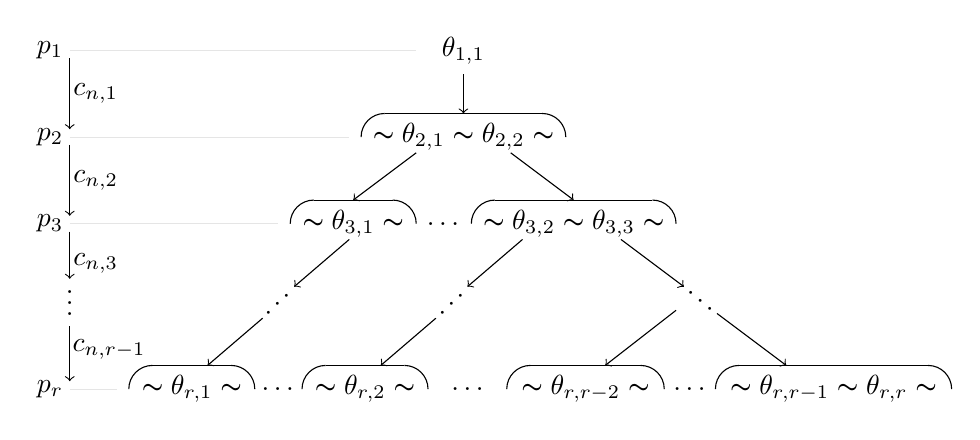
\begin{tikzpicture}
		\newcommand{\halfblob}[5]{ % #1: radius, #2: half-length, #3: x-coordinate, #4: y-coordinate, #5: name
			\draw (#3 - #2,#4 + #1) arc [start angle=90, end angle=180, radius=#1];
			\draw (#3 + #2 + #1,#4) arc [start angle=0, end angle=90, radius=#1];
			\draw (#3 - #2,#4 + #1) -- (#3 + #2,#4 + #1);
			%\draw (#3 - #2,#4 - #1) -- (#3 + #2,#4 - #1);
			\node at (#3,#4) {#5};
		}
		
		\node at (0,0) {$\theta_{1,1}$};
		\draw[->] (0,-0.3) -> (0,-0.8);
		\halfblob{0.3}{1}{0}{-1.1}{$\thicksim \theta_{2,1} \thicksim \theta_{2,2} \thicksim$}
		
		\draw[->] (-0.6,-1.3) -> (-1.4,-1.9);
		\halfblob{0.3}{0.5}{-1.4}{-2.2}{$\thicksim \theta_{3,1} \thicksim$}
		\draw[->] (0.6,-1.3) -> (1.4,-1.9);
		\halfblob{0.3}{1}{1.4}{-2.2}{$\thicksim \theta_{3,2} \thicksim \theta_{3,3} \thicksim$}
		\node at (-0.23,-2.2) {$\dots$};
		
		\draw[->] (-1.45,-2.4) -> (-2.15,-3);
		\node[rotate=43] at (-2.34,-3.2) {$\dots$};
		\draw[->] (-2.55,-3.4) -> (-3.25,-4);
		\halfblob{0.3}{0.5}{-3.45}{-4.3}{$\thicksim \theta_{r,1} \thicksim$}
		
		\draw[->] (0.75,-2.4) -> (0.05,-3);
		\node[rotate=43] at (-0.13,-3.2) {$\dots$};
		\draw[->] (-0.35,-3.4) -> (-1.05,-4);
		\halfblob{0.3}{0.5}{-1.25}{-4.3}{$\thicksim \theta_{r,2} \thicksim$}
		
		\draw[->] (2,-2.4) -> (2.8,-3);
		\node[rotate=-40] at (3.03,-3.2) {$\dots$};
		\draw[->] (2.7,-3.3) -> (1.8,-4);
		\halfblob{0.3}{0.7}{1.55}{-4.3}{$\thicksim \theta_{r,r-2} \thicksim$}
		\draw[->] (3.22,-3.34) -> (4.1,-4);
		\halfblob{0.3}{1.2}{4.7}{-4.3}{$\thicksim \theta_{r,r-1} \thicksim \theta_{r,r} \thicksim$}
		
		\node at (-2.33,-4.3) {$\dots$};
		\node at (0.08,-4.3) {$\dots$};
		\node at (2.9,-4.3) {$\dots$};
		
		%vertical arrows on the side
		\draw[->] (-5,-0.1) -> (-5,-1);
		\node at (-4.67,-0.55) {$c_{n,1}$};
		\draw[->] (-5,-1.2) -> (-5,-2.1);
		\node at (-4.67,-1.65) {$c_{n,2}$};
		\draw[->] (-5,-2.3) -> (-5,-2.9);
		\node at (-4.67,-2.7) {$c_{n,3}$};
		\node at (-5,-3.1) {$\vdots$};
		\draw[->] (-5,-3.5) -> (-5,-4.2);
		\node at (-4.5,-3.8) {$c_{n,r-1}$};
		
		%horizontal gray lines
		\draw[gray!20] (-5,0) -> (-0.6,0);
		\draw[gray!20] (-5,-1.1) -> (-1.45,-1.1);
		\draw[gray!20] (-5,-2.2) -> (-2.35,-2.2);
		\draw[gray!20] (-5,-4.3) -> (-4.4,-4.3);
		
		%look-ahead states
		\node at (-5.25,0) {$p_1$};
		\node at (-5.25,-1.1) {$p_2$};
		\node at (-5.25,-2.2) {$p_3$};
		\node at (-5.25,-4.3) {$p_r$};		
		
	\end{tikzpicture}
\end{center}
Note that, in this representation, we chose to represent 
$\theta_{i,i} \to_{c_i} w_{i} \, \theta_{i+1,i} \, w'_{i} \, \theta_{i+1,i+1} \, w''_i$ instead of 
$\theta_{i,i} \to_{c_i} w_{i} \, \theta_{i+1,i+1} \, w'_{i} \, \theta_{i+1,i} \, w''_i$ for all $i \in [r-1]$. 
But this distinction does not matter to the proof of the claim. 
%but because the order of nesting does not matter for nesting loops, 
%we can assume that branching is happening on the right without loss of generality (in fact 
%branching on the left makes the proof easier by excluding the case where $\bot$ occurs on the branching side). 
From now on we use $\thicksim$ to denote arbitrary sequences in $\QY^*$ which we will not use to find a nesting loop. 

\begin{proof}
We prove this by induction on $r$. 
Let $c$ be a $\Sigma$-context, $\theta$ a pair in $\QY$ and $w$ a sequence in $\QY^*$ with $\theta \to_{c} w$ and $|w| \geq B^{r+1}$. 
We split $c$ into atomic $\Sigma$-contexts $c'_1, \dots, c'_n$, then we have sequences $w_1, \dots, w_{n-1} \in \QY^*$ 
such that $\theta \to_{c'_1} w_1 \dots \to_{c'_{n-1}} w_{n-1} \to_{c'_n} w$. 
Let $i$ be the largest $i$ such that there is a pair $\theta'$ in sequence $w_i$ with $\theta' \to_{c'_{i+1} \cdots c'_n} w'$ and $|w'| \geq B^r$. 
If we had $|w'| \geq B^{r+1}$ then, because $c'_{i+1}$ is atomic, we would have a $\theta''$ in sequence $c'_{i+1}$ with $\theta'' \to_{c'_{i+2} \cdots c'_n} w''$ and $|w''| \geq B^r$. 
So $B^r \leq |w'| < B^{r+1} \leq |w|$. 
Therefore there is another pair $\theta_{2,1}$ in $w_i$ (other than $\theta'$) with $\theta_{2,1} \to_{c'_{i+1} \cdots c'_n} w''$ and $|w''| \geq 1$. 

Since $\theta' \to_{c'_{i+1} \cdots c'_n} w'$ and $|w'| \geq B^r$, we use the induction hypothesis on $theta'$ and $c'_{i+1} \cdots c'_n$. In order to prove the induction for $r+1$, we rename the $\Sigma$-contexts $c_1, \dots c_{r-1}$, look-ahead states $p_1, \dots, p_r$ and pairs $\theta_{i,j}$ (for $j \leq i \leq r$) into $\Sigma$-contexts $c_2, \dots c_{r}$, look-ahead states $p_2, \dots, p_{r+1}$ and pairs $\theta_{i+1,j+1}$ (for $j \leq i \leq r$). 
Then $c'_{i+1} \cdots c'_n = c_2 \cdots c_{r}$. 

Since $\theta_{2,1} \to_{c_2 \cdots c_r} w''$ with $|w''| \geq 1$, there are pairs $\theta_{3,1}, \dots, \theta_{n,1}$ such that $\theta_{n,1}$ appears in sequence $w''$ and, for all $i \in [r]$ with $i \geq 2$, $\theta_{i,1} \to_{c_i} w'_i \, \theta_{i+1,1} \, w''_i$ with $w'_i, w''_i \in \QY^*$. 
To conclude, we choose $c_1 = c'_1 \dots c'_i$, $p_1 = h(c_1)$ and $\theta_{1,1} = \theta$. 
\end{proof}

In order to find a nesting loop, we need two indexes $i$ and $j$ with: 
\begin{center}
	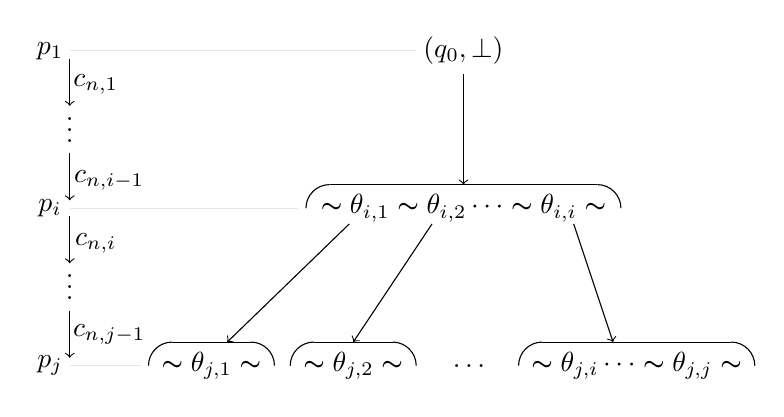
\begin{tikzpicture}
		\newcommand{\halfblob}[5]{ % #1: radius, #2: half-length, #3: x-coordinate, #4: y-coordinate, #5: name
			\draw (#3 - #2,#4 + #1) arc [start angle=90, end angle=180, radius=#1];
			\draw (#3 + #2 + #1,#4) arc [start angle=0, end angle=90, radius=#1];
			\draw (#3 - #2,#4 + #1) -- (#3 + #2,#4 + #1);
			%\draw (#3 - #2,#4 - #1) -- (#3 + #2,#4 - #1);
			\node at (#3,#4) {#5};
		}
		
		\node at (0,0) {$(q_0,\bot)$};
		\draw[->] (0,-0.3) -> (0,-1.7);
		\halfblob{0.3}{1.7}{0}{-2}{$\thicksim \theta_{i,1} \thicksim \theta_{i,2} \dots \thicksim \theta_{i,i} \thicksim$}
		
		\draw[->] (-1.45,-2.2) -> (-3,-3.7);
		\halfblob{0.3}{0.5}{-3.2}{-4}{$\thicksim \theta_{j,1} \thicksim$}
		
		\draw[->] (-0.4,-2.2) -> (-1.4,-3.7);
		\halfblob{0.3}{0.5}{-1.4}{-4}{$\thicksim \theta_{j,2} \thicksim$}
		
		\draw[->] (1.4,-2.2) -> (1.9,-3.7);
		\halfblob{0.3}{1.2}{2.2}{-4}{$\thicksim \theta_{j,i} \dots \thicksim \theta_{j,j} \thicksim$}
		\node at (0.1,-4) {$\dots$};
		
		%vertical arrows on the side
		\draw[->] (-5,-0.1) -> (-5,-0.7);
		\node at (-4.67,-0.43) {$c_{n,1}$};
		\node at (-5,-0.9) {$\vdots$};
		\draw[->] (-5,-1.3) -> (-5,-1.9);
		\node at (-4.5,-1.65) {$c_{n,i-1}$};

		\draw[->] (-5,-2.1) -> (-5,-2.7);
		\node at (-4.67,-2.45) {$c_{n,i}$};
		\node at (-5,-2.9) {$\vdots$};
		\draw[->] (-5,-3.3) -> (-5,-3.9);
		\node at (-4.5,-3.6) {$c_{n,j-1}$};
		
		%horizontal gray lines
		\draw[gray!20] (-5,0) -> (-0.6,0);
		\draw[gray!20] (-5,-2) -> (-2.1,-2);
		\draw[gray!20] (-5,-4) -> (-4.1,-4);
		
		%look-ahead states
		\node at (-5.25,0) {$p_1$};
		\node at (-5.25,-2) {$p_i$};
		\node at (-5.25,-4) {$p_j$};		
		
	\end{tikzpicture}
\end{center}
Formally, we require two indexes $i,j$ with $i < j < r$ which share the same:
\begin{itemize}
\item look-ahead state $h(c_{n,i}) = h(c_{n,j})$, 
\item pair $\theta_{i,i} = \theta_{j,j} \in \QY$, 
\item set of pairs $\{\theta_{i,\ell}\}_{0\leq \ell \leq i} = \{\theta_{j,\ell}\}_{0\leq \ell \leq j}$.  
\end{itemize}
We ensure the existence of such $i,j$ by taking $r \geq |P|\,|Q|\,(m+1) \, 2^{|Q| (m+1)} +1$ 
%(so $n = B^{|P|\,|Q|\,(m+1)\, 2^{|Q| (m+1)} +1}$) 
where $m$ is the maximum arity of states. 
%We ensure the existence of such $i,j$ by taking $r \geq |P|\,|\QY| \, 2^{|\QY|} +1$ 
%(so $n = B^{|P|\,|\QY|\, 2^{|\QY|} +1}$) with $|\QY| \leq |Q| \, (m+1)$ where $m$ is the maximum arity of states. 
We now show how to build the nesting loop from indexes $i,j$. 
We note $p = h(c_{n,i}) = h(c_{n,j})$, $(q_1,k_1) = \theta_{i,i} = \theta_{j,j}$ and 
$S = \{\theta_{i,\ell}\}_{0\leq \ell \leq i} = \{\theta_{j,\ell}\}_{0\leq \ell \leq j}$. 
We note $c' = c_{n,i}.c_{n,i+1}. \dots. c_{n,j-1}$. 
Note that $c'$ has a leaf labeled $p$ and $h(c')=p$. 
%drawing maybe

We need the sets $\{\theta_{i,\ell}\}_{0\leq \ell \leq i}$ and $\{\theta_{j,\ell}\}_{0\leq \ell \leq j}$ 
to be equal so that the pairs $\theta_{i,k}$ for $k \leq i$ loop on each other through the loop $c'$. 
Formally, noting $\theta'_0 = \theta_{j,i}$, for all $\theta'_k \in S$ for $k \in \N$, there exists 
$\theta'_{k+1} \in S$ such that $\theta'_k \to_c' \,\thicksim \theta'_{k+1} \thicksim$. 
Since $S \subseteq \QY$ is finite, there must be $n, m \in \N$ such that 
$\theta'_{n} = \theta'_{n+m}$ (with $m \geq 1$), so $\theta'_n \to_{c'^m} \,\thicksim \theta'_n \thicksim$. 
Also $(q_1,k_1) \to_{c'} \,\thicksim \theta'_0 \thicksim (q_1,k_1) \thicksim\,$ and $\theta'_0 \to_{c'^n} x_n$, 
so $(q_1,k_1) \to_{c'^{n+1}} \, \thicksim \theta'_n \thicksim (q_1,k_1) \thicksim\,$ and, for all $m' \in \N$: 
$(q_1,k_1) \to_{c'^{m'}} \, \thicksim (q_1,k_1) \thicksim \, \to_{c'^{n+1}} \, \thicksim \theta'_n \thicksim (q_1,k_1) \thicksim$. 
Finally, for $c = c'^{m(n+1)}$, we have 
$(q_1,k_1) \to_{c} \, \thicksim \theta'_n \thicksim (q_1,k_1)\thicksim$ and $\theta'_n \to_{c} \theta'_n$. 
So we have a \emph{nesting loop}. 

In conclusion, if $M$ is not finite nesting, then it is \emph{nested input pumpable}, and so it does not have linear size-to-height increase. 
\vspace{2mm}

The proof of Statement~(2) can be given in a very similar way as for~(1), here we only outline the changes to the notations which allow to adapt the proof of~(1) to~(2). 
We replace $\Sigma$-contexts with elements of the set $T_\Sigma(P)$ containing possibly several leafs labeled in $P$. The rest of the notational changes are consequences of this change. 
Given a $s \in T_\Sigma(P)$, we now consider the nesting of state calls called on distinct subtrees of $s$ with potentially distinct look-ahead states. We augment pairs in $\QY$ so as to include the look-ahead, so $\QY = \{ (q,k,p) \mid q \in Q^{(m)}, k \in [m] \cup \{\bot\}, p \in P\}$. The notation $(q,k,p) \to_s (q_1,k_1,p_1) \dots (q_n,k_n,p_n)$ means that $h(s)=p$ and calls to states $q_1, \dots, q_n$ on leafs of $s$ labeled $p_1, \dots, p_n$ resp.\ are nested on parameters $y_{k_1}, \dots, y_{k_n}$ along a path in $\widehat{M}_q(s)$. This means that, when concatenating contexts, we write $s(s_1, \dots, s_m)$ instead of $s\cdot s'$. 

For~(2), similarly to nesting loops for~(1), we define a \emph{yield nesting loop} as given by contexts $s_1, s_2 \in T_\Sigma(P)$, look-ahead states $p_1, p_2 \in P$ and triplets $(q_1,k_1,p_1), (q_2,k_2,p_2) \in \QY$ such that:
\begin{itemize}
\item $h(s_1) = p_1$, $h(s_2) = p_2$, $s_1$ has two leafs labeled $p_1$ and $p_2$, $s_2$ has one leaf labeled $p_2$, 
\item $\<q_1,p_1>$ is reachable, 
\item either $(q_1,k_1,p_1) \to_{s_1} \thicksim\, (q_2,k_2,p_2) \,\thicksim\, (q_1,k_1,p_1) \,\thicksim$ \\
\phantom{.} \hspace{2.5mm} or $(q_1,k_1,p_1) \to_{s_1} \thicksim\, (q_1,k_1,p_1) \,\thicksim\, (q_2,k_2,p_2) \,\thicksim$,
\item $(q_2,k_2,p_2) \to_{s_2} \thicksim\, (q_2,k_2,p_2) \,\thicksim$. 
\end{itemize}
  
We say that $M$ is \emph{yield nested input pumpable} when it has either a \emph{yield nesting loop} or a \emph{nesting loop}. 
Note that the existence of either of these loops falsifies the linear height increase property. 
To prove~(2) we prove that infinite yield nesting implies the existence of either a yield nesting loop or a nesting loop. That proof works similarly to~(1): $M$ is not fynest so we can find large enough nesting sequences (but with the new definition of $\to_s$), find a repeating triplet $(q_1,k_1,p_1)$, pump the loop enough times that a triplet $(q_2,k_2,p_2)$ loops onto itself. Note that if the nested calls to $(q_1,k_1,p_1)$ and $(q_2,k_2,p_2)$ in $(q_1,k_1,p_1) \to_{s_1} \,\thicksim (q_2,k_2,p_2) \thicksim (q_1,k_1,p_1) \thicksim$ are on the same leaf in $s_1$ (with $p_1 = p_2$), then we get a nesting loop (otherwise we get a yield nesting loop). 



%%old version of definition of \to_s
%(Old version.) When considering the nesting of states, we want to specify the look-ahead the state is called upon, and in which parameter the nesting occurs. We define the set $\QY = \{ (q,p,y_k) \mid q \in Q^{(m)}, p \in P, y_k \in Y_m \cup \{\bot\}\}$ of nesting state configurations. We use configuration $(q,p,\bot)$ to denote the state called at the bottom of a nesting chain, with no state calls in any of its parameters. 
%
%For a $\Sigma$-context $s$ containing a leaf $p$, we write $(q,h(s),\bot) \to_s (q_1,p,y_{k_1}) \dots (q_{n-1},p, y_{k_{n-1}}) (q_n,p,\bot)$ when state calls $\<q_1,p>, \<q_2,p>, \dots$ appear nested in $M_{q}(s)$, with $\<q_2,p>$ appearing in parameter $y_{k_1}$ of $\<q_1,p>$, $\<q_3,p>$ appearing in parameter $y_{k_2}$ of $\<q_2,p>$ and so on. We write $(q,h(s),y_k) \to_s (q_1,p,y_{k_1}) \dots (q_n,p,y_{k_n})$ when $(q,h(s),\bot) \to_s (q_1,p,y_{k_1}) \dots (q_{n-1},p, y_{k_{n-1}}) (q_n,\bot)$ and parameter $y_k$ of $q$ appears in parameter $y_{k_n}$ of $\<q_n,p>$. 
%%For a $\Sigma$-context $s$ containing look-ahead state $p$, we write $(q_0,p_0,y_{k_0}) \to_s (q_1,p,y_{k_1}) \dots (q_n,p,y_{k_n})$ when $p_0 = h(s)$ and, in $M_{q_0}(s)$, state calls $\<q_1,p>, \<q_2,p>, \dots$ appear nested on parameters $y_{k_1}, y_{k_2}, \dots$, along a path leading to parameter $y$. 
%%We write $(q_0,p_0,\bot) \to_s (q_1,p,x_1) \dots (q_n,p,x_n)$ when $p_0 = h(s)$ and there exists exactly one $x_i$ with $x_i = \bot$ such that, in $M_{q_0}(s)$, state calls $\<q_1,p>, \dots$ appear nested on parameters $y_{k_1}, y_{k_2}, \dots$, along a path leading to parameter $y$. 
%Note that $\to_s$ is closed under subsequence on the right (i.e.\ we can "forget" part of the nested configurations). 
%We extend the relation $\to_s$ so that it is commutative and compatible with concatenation of sequences in $\QY^*$, i.e.\ so that $w \to_s w_2 w_1$ when $w \to_s w_1 w_2$, and $w_1 w_2 \to_s w'_1 w'_2$ when both $w_1 \to_s w'_1$ and $w_2 \to_s w'_2$, for all $w, w_1, w'_1, w_2, w'_2 \in \QY^*$. 
%Given two $\Sigma$-contexts $s$ and $s'$ containing look-ahead states $p$ and $p'$, if $p = h(s')$, then $s\cdot s'$ denotes the $\Sigma$-context obtained from $s$ by replacing $p$ with $s'$. Note that, for all $a \in \QY$ and $w \in \QY^*$, $a \to_{s\cdot s'} w$ if and only if there exists $w' \in \QY^*$ such that $a \to_s w'$ and $w' \to_{s'} w$. 
%%We sometimes write $\to$ instead of $\to_s$ when $s$ is obvious from context or does not matter. 
%
%
%%definition of nesting loops
%(Definition of nesting loops.) We can now define \emph{nesting loops}, whose existence characterizes \emph{nested input pumpability}. 
%A \emph{nesting loop} is given by a $\Sigma$-context $s$ and two configurations $(q_1,p,y_i)$ and $(q_2,p,y_j) \in \QY$ such that: $\<q_1,p>$ is reachable, $(q_1,p,y_i) \to_s (q_2,p,y_j) (q_1,p,y_i)$ and $(q_2,p,y_j) \to_s (q_2,p,y_j)$. Note that $y_i$ could be either $\bot$ or a parameter of $q_1$ (these two cases represent the two cases in point 2. of the definition of nested input pumpability), but in either case $y_j \neq \bot$. 
%
%
%%\begin{claim}
%%If $M$ has a nesting loop then $M$ is not of linear size-to-height increase. 
%%\end{claim}
%%
%%\begin{proof}
%%We prove this by pumping the loop: pumping $n$ times gives either $(q_1,y_i) \to_{s^n} (q_1,y_i) (q_2,y_j)^n$ or $(q_1,y_i) \to_{s^n} (q_2,y_j)^n (q_1,y_i)$. Since $\<q_1,p>$ is reachable, there exists a $\Sigma$-context $s_0$ which leads to the state call $\<q_1,p>$. For all input tree $t \in L_p$, the output of $M$ on input $s_0(s^n(t))$ nests $n$ calls to state $q_2$ on tree $t$ (nested along parameter $y_j$). The input size is $|s_0| + n.|s| + |t|$ and the output height is at least $n.d$ where $d$ is the maximum depth of parameter $y_j$ in $q_2(t)$. 
%%If $M$ was of linear size-to-height increase we would have a bound $B$ such that $B.(|s_0| + n.|s| + |t|)\geq n.d$ for all $n$, so $B.|s| \geq d$. 
%%Since $M$ is depth proper, there is no upper bound for the depth $d$ where $y_j$ occurs in $q_2(t)$ for $t \in L_p$, so $M$ can not be of linear size-to-height increase. 
%%\end{proof}
%
%We now only need to prove that if $M$ is not finite nesting then it has a nesting loop. We assume that $M$ is not finite nesting, so for all $n \in \N$ there exists a $Sigma$-context $s$ and a configuration sequence $w \in \QY^n$ such that $(q_0,h(s),\bot) \to_s w$. We decompose $\Sigma$-context $s$ into a concatenation $s_1\cdot s_2\cdot \dots \cdot s_k$ of atomic $\Sigma$-contexts (i.e.\ context whose hole is at depth $1$) and we get: 
%$(q_0,h(s),\bot) \to_{s_1} x_{1,1} \dots x_{1,m_1} \to_{s_2} \dots \to_{s_m} x_{k,1} \dots x_{k,m_k}$ with $x_{i,j} \in \QY$ for all $i,j$ and $m_k = n$. 
%We can represent this structure of nested state calls as a \emph{configuration tree}:
%%tikz picture: configuration tree: $(q_0,h(s),\bot) \to_{s_1} x_{1,1} \dots x_{1,m_1} \to_{s_2} \dots \to_{s_m} x_{k,1} \dots x_{k,m_k}$
%%% Figure environment removed
%
%We say that a configuration tree is a $k$-comb if it is of the form:
%%tikz picture: $k$-comb
%\begin{center}
%\begin{tikzpicture}
%\node {$(q_0,p_0,\bot)$} [sibling distance = 12mm, level distance = 9mm]
%child {node {$x_{1,1}$}
%	child {node {$x_{2,1}$}
%		child {node {$x_{3,1}$}
%			child {node[rotate=57] {$\dots$}
%				child {node {$x_{k,1}$}
%				}
%				child[missing]
%			}
%			child[missing]
%		}
%		child[missing]
%	}
%	child {node {$x_{2,2}$}
%		child {node {$x_{3,2}$}
%			child {node[rotate=57] {$\dots$}
%				child {node {$x_{k,2}$}
%				}
%				child[missing]
%			}
%			child[missing]
%		}
%		child {node {$x_{3,3}$}
%			child {node[rotate=57] {$\dots$}
%			}
%			child {node[rotate=-57] {$\dots$}
%				child {node {$x_{k,k-1}$}
%				}
%				child {node {$x_{k,k}$}
%				}
%			}
%		}
%	}
%}
%;
%\node at (0,-4.5) {$\dots$};
%
%%other version:
%%\node {$(q_0,p_0,\bot)$} [sibling distance = 12mm, level distance = 10mm]
%%child {node {$x_{1,1}$}
%%	child {node {$x_{2,1}$}
%%		child {node[rotate=58] {$\dots$}
%%			child {node {$x_{k-1,1}$}
%%				child {node {$x_{k,1}$}
%%				}
%%				child[missing]
%%			}
%%			child[missing]
%%		}
%%		child[missing]
%%	}
%%	child {node {$x_{2,2}$}
%%		child {node[rotate=58] {$\dots$}
%%			child {node {$x_{k-1,2}$}
%%				child {node {$x_{k,2}$}
%%				}
%%				child[missing]
%%			}
%%			child[missing]
%%		}
%%		child {node[rotate=-58] {$\dots$}
%%			child[missing]
%%			child {node {$x_{k-1,k-1}$}
%%				child {node {$x_{k,k-1}$}
%%				}
%%				child {node {$x_{k,k}$}
%%				}
%%			}
%%		}
%%	}
%%}
%%;
%%\node at (0,-5) {$\dots$};
%\end{tikzpicture}
%\end{center}
%\vspace{-2mm}
%
%In configuration trees obtained by decomposing a $\Sigma$-context into atomic contexts, nodes have their arity bound by the nesting on the right-hand-side of rules of $M$. Noting this bound $B$, and for all $k \in \N$, any configuration tree with $B^{k+1}$ leafs and obtained by atomic decomposition can be pruned into a $k$-comb. 
%
%Formally, we prove this by induction on $k$. The allowed pruning operations are: $(a)$ remove a node and all its descendants, $(b)$ remove all nodes at a given depth by merging them with their parent node. Note that the nesting statements represented by the trees remain true when pruned. Also, pruned trees preserve the property: for all depth $i<k$, noting $x_{i,1}, \dots, x_{i,m_i}$ the nodes at depth $i$ and $x_{i+1,1}, \dots, x_{i+1,m_{i+1}}$ the nodes at depth $i+1$, there is a $\Sigma$-context $s_i$ such that:
%\vspace{-2mm}
%
%\[x_{i,1} \dots x_{i,m_i} \to_{s_i} x_{i+1,1} \dots x_{i+1,m_{i+1}}\]
%\vspace{-3mm}
%
%We now argue that by taking a big enough $k$-comb we ensure the existence of a nesting loop. We take $k= |\QY|.2^{|\QY|} +1$. Such a $k$-comb must have two depths $i,j$ with $i<j\leq k$ which share the same: 
%\begin{enumerate}
%\item configuration $(q_1,p,y_i) = x_{i,i} = x_{j,j}$ (the configuration on the spine of the comb, i.e.\ the right-most node at depth $i$ and $j$), 
%\item set of configurations $S= \{x_{i,\ell}\}_{0\leq \ell \leq i} = \{x_{j,\ell}\}_{0\leq \ell \leq j}$ (the sets of all configurations appearing at depth $i$ and $j$). 
%\end{enumerate}
%%Note that $k= |\QY|.2^{|\QY|/ |P|} +1$, where $|P|$ is the number of look-ahead states, would be enough because nodes of a same depth have the same $p$, but when adapting this proof to point~(2) we would need $k= |\QY|.2^{|\QY|} +1$. 
%So we have a $\Sigma$-context $s$ such that $(q_1,p,y_i) \to_s w_3 (q_1,p,y_i)$ and $w_1 \to_s w_2$ with $w_1, w_2, w_3 \in S^*$ and all configuration $x \in S \setminus \{(q_1,p,y_i)\}$ appears at least once in $w_1$ and once in $w_2 w_3$: 
%% tikzpicture of the loop s
%\begin{center}
%\begin{tikzpicture}
%\node at (-2,0) {$\phantom{B}$} [sibling distance = 12mm, level distance = 9mm]
%child {node[rotate=55] {$\dots$}
%	child {node {$\phantom{B}$}}
%	child[missing]
%}
%child[missing]
%;
%
%\node {$\phantom{B}$} [sibling distance = 12mm, level distance = 9mm]
%child {node[rotate=55] {$\dots$}
%	child {node {$\phantom{B}$}}
%	child[missing]
%}
%child[missing]
%;
%
%\node at (1,0) {$(q_1,p,y_i)$} [sibling distance = 12mm, level distance = 9mm]
%child {node[rotate=55] {$\dots$}
%	child {node {$\phantom{B}$}}
%	child[missing]
%}
%child {node[rotate=-55] {$\dots$}
%	child {node {$\phantom{B}$}}
%	child {node {$(q_1,p,y_i)$}}
%}
%;
%
%\newcommand{\blobby}[5]{ % #1: radius, #2: x1-coordinate, #3: x2-coordinate, #4: y-coordinate, #5: name
%	\draw (#2,#4 + #1) arc [start angle=90, end angle=270, radius=#1];
%	\draw (#3,#4 - #1) arc [start angle=-90, end angle=90, radius=#1];
%	\draw (#2,#4 + #1) -- (#3,#4 + #1);
%	\draw (#2,#4 - #1) -- (#3,#4 - #1);
%	\node at ($(#2,#4)!0.5!(#3,#4)$) {#5};
%}
%
%\blobby{0.23}{-2}{0}{0}{$w_1$}
%\blobby{0.23}{-3.2}{-1.2}{-1.8}{$w_2$}
%\blobby{0.23}{-0.2}{1}{-1.8}{$w_3$}
%
%\node at (-1.55,-0.9) {$\dots$};
%\end{tikzpicture}
%\end{center}
%
%Let $x_0 \in S$ be a configuration in $w_3$ (we can do so because $|w_3| = j-i \geq 1$). 
%Because $w_1 \to_s w_2$, we know that each configuration $x_k \in S$ has a $x_{k+1} \in S$ such that $x_k \to_s x_{k+1}$. Because $S \subseteq \QY$ is finite, there must be $n, m \in \N$ such that $x_{n} = x_{n+m}$ (with $m \geq 1$), so $x_n \to_{s^m} x_n$. Also $(q_1,p,y_i) \to_s (q_1,p,y_i)\, x_0$ and $x_0 \to_{s^n} x_n$, so $(q_1,p,y_i) \to_{s^{n+1}} (q_1,p,y_i)\, x_n$ and, for all $m' \in \N$: $(q_1,p,y_i) \to_{s^{m'}} (q_1,p,y_i) \to_{s^{n+1}} (q_1,p,y_i)\, x_n$. Finally, for $s_\ell = s^{m(n+1)}$, we have $(q_1,p,y_i) \to_{s_\ell} (q_1,p,y_i)\, x_n$ and $x_n \to_{s_\ell} x_n$. So we have a \emph{nesting loop}. 
%
%In conclusion, if $M$ is not finite nesting, then it is \emph{nested input pumpable}, and so it does not have linear size-to-height increase. 
%\vspace{2mm}

%The proof of Statement~(2) can be given in a very similar way as for~(1), here we only outline the changes to the notations which allow to adapt the proof of~(1) to~(2). 
%First we replace $\Sigma$-contexts with regular contexts (i.e.\ elements of the set $T_\Sigma(P)$) containing possibly several leafs in $P$. The rest of the notational changes are consequences of this change. 
%For $s \in T_\Sigma(P)$, the notation $(q,p,y) \to_s (q_1,p_1,y_{k_1}) \dots (q_n,p_n,y_{k_n})$ means that calls to states $q_1, \dots, q_n$ are nested along a path in $M_q(s)$, but now these calls can be on different leafs of $s$. This means that, when concatenating contexts, we use $s(s_1, \dots, s_m)$ instead of $s\cdot s'$. 
%
%For~(2), similarly to nesting loops for~(1), we define a \emph{yield nesting loop} as given by a pair of contexts $s_1, s_2 \in T_\Sigma(P)$, and configurations $(q_1,p_1,y_i), (q_2,p_2,y_j) \in \QY$ such that: $\<q_1,p_1>$ is reachable, $(q_1,p_1,y_i) \to_{s_1} (q_2,p_2,y_j) (q_1,p_1,y_i)$, and $(q_2,p_2,y_j) \to_{s_2} (q_2,p_2,y_j)$. 
%We say that $M$ is \emph{yield nested input pumpable} when it has either a \emph{yield nesting loop} or a \emph{nesting loop}. 
%Note that the existence of either of these loops falsifies the linear height increase property. 
%To prove~(2) we prove that infinite yield nesting implies the existence of either a yield nesting loop or a nesting loop. That proof works similarly to~(1): existence of $k$-combs for any $k$ (but with the new definition of $\to_s$), find a repeating configuration $(q_1,p_1,y_i)$ on the spine of the comb, pump the loop enough times that a configuration $(q_2,p_2,y_j)$ comes onto itself. Note that if the nested calls to $(q_1,p_1,y_i)$ and $(q_2,p_2,y_j)$ in $(q_1,p_1,y_i) \to_{s_1} (q_2,p_2,y_j)\, (q_1,p_1,y_i)$ are on the same leaf in $s_1$, then we get a nesting loop (otherwise we get a yield nesting loop). 

%
%%Paul's version
%Because $M$ is depth-proper, for each $q \in Q^{(m)}, i \in [m], p \in P$ and 
%$n \in \N$, there is $t \in L_p$ such that $\he{\lcop{M_q(t)}_{\{y_i\}}} > n$. 
%We can ensure the existence of a productive loop in $t$ by taking 
%$n = 1+ \text{mhr} . k^{|Q| . |P|}$ where $k$ is the maximum arity of input trees. 
%Noting $t_j$ the tree where the loop is pumped $j$ times, we get 
%\[\he{\lcop{M_q(t_j)}_{\{y_i\}}} > c_s.|t_j| ~~~~\text{ and }~~~~ 
%\he{\lcop{M_q(t_j)}_{\{y_i\}}} > c_h.\he{t_j}\] 
%for all $j \geq 1$, 
%where $c_s$ and $c_h$ are strictly positive constants that depend on $M, q, i$ and $p$. 
%We can make $c_s$ and $c_h$ only dependent on $M$ by taking their maximum over 
%the possible $q \in Q^{(m)}, i\in [m]$ and $p \in P$. 
%
%To prove~(1), assume that $M$ is not fnest.
%We will show that this implies that $M$ does not have LSHI.
%For all $n \in \N$, there is $s \in T_\Sigma(P)$ with one occurrence of $P$ 
%such that there are at least $n$ nested occurrences of $P$ in $\he{\hat{M}(s)}$. 
%By taking $n$ big enough, we can get any number of nested calls of 
%\emph{the same state} $q$, nested in \emph{the same parameter} $y_i$ of $q$. 
%For all $n \in \N$, we note $s_{n} \in T_\Sigma(P)$ the tree with one occurrence of $P$ 
%such that there are at least $n$ occurrences of 
%$\langle q,p \rangle$ nested along parameter $y_i$ in $\he{\hat{M}(s)}$, 
%for some $q \in Q^{(m)}, i \in [m]$ and $p \in P$. We note $u_n$ such that $s_n/u_n \in P$, 
%and $t_{n,j} = s_n[u_n \leftarrow t_j]$ for all $n,j \in \N$. 
%For each $n$, there is $j_n$ such that $|t_{j_n}| > |s_n|$, so $|t_{j_n}| > |t_{n,j_n}|/2$. 
%Then, for all $n \in \N$:
%\[\he{M(t_{n,j_n})} \geq n.\he{\lcop{M_q(t_{j_n})}_{\{y_i\}}} > n.c_s.|t_{j_n}| > n.c_s.|t_{n,j_n}|/2 \]
%If $M$ had LSHI then there would be a constant $c$ such that \\
%$c > \he{M(t_{n,j_n})}/|t_{n,j_n}| > n.c_s/2$ for all $n \in \N$. 
%This is a contradiction, so $M$ does not have LSHI. 
%
%To prove~(2), assume that $M$ is not fynest.
%We will show that this implies that $M$ does not have LHI.
%For all $n \in \N$, there is $s \in T_\Sigma(P)$ 
%such that there are at least $n$ nested occurrences of $P$ in $\he{\hat{M}(s)}$. 
%By taking $n$ big enough, we can get any number of nested calls of 
%\emph{the same state} $q$, nested in \emph{the same parameter} $y_i$ of $q$, 
%applied to \emph{the same look-ahead state} $p$. 
%For all $n \in \N$, we note $s_{n} \in T_\Sigma(P)$ the tree 
%such that there are at least $n$ occurrences of 
%$\langle q,p \rangle$ nested along parameter $y_i$ in $\he{\hat{M}(s)}$, 
%for some $q \in Q^{(m)}, i \in [m]$ and $p \in P$. 
%We note $t_{n,j} = s_n[p \leftarrow t_j]$ for all $n,j \in \N$. 
%For each $n$, there is $j_n$ such that $\he{t_{j_n}} > \he{s_n}$, so $\he{t_{j_n}} > \he{t_{n,j_n}}/2$. 
%Then, for all $n \in \N$:
%\[\he{M(t_{n,j_n})} \geq n.\he{\lcop{M_q(t_{j_n})}_{\{y_i\}}} > n.c_h.\he{t_{j_n}} > n.c_h.\he{t_{n,j_n}}/2 \]
%If $M$ had LHI then there would be a constant $c$ such that \\
%$c > \he{M(t_{n,j_n})}/\he{t_{n,j_n}} > n.c_h/2$, for all $n \in \N$.
%This is a contradiction, so $M$ does not have LHI. 
%
%\qed
\end{proof}

From Theorem~\ref{th:proper} and Lemmas~\ref{lm:decidable},~\ref{lm:easy}, and~\ref{lm:nest} we obtain
our following main theorem.

\begin{theorem}
Let $M$ be an mttr. 
Then 
(1)~it is decidable whether or not $M$ has linear size-to-height increase
(2)~it is decidable whether or not $M$ is linear height-increase.
\end{theorem}

%% -*- mode: LaTeX; fill-column: 78; -*-

\section{Concluding Remarks}
\label{sec:conclusions}

In this paper, we presented a novel SMC algorithm, \EventDPOR, tailored to the
characteristics of event-driven multi-threaded programs running under the SC
semantics. The algorithm was proven correct and optimal for event-driven
programs in which the variable accesses of events do not depend on how their
execution is interleaved with other threads.

We have implemented \EventDPOR in the \Nidhugg tool, and we will open-source
our implementation.
%
With a wide range of event-driven programs, we have shown that \EventDPOR
incurs only a moderate constant overhead over its baseline implementation
(\OptimalDPOR), it is exponentially faster than existing state-of-the-art SMC
algorithms in time and number of traces examined on programs where events'
actions do not conflict, and does not suffer from performance degradation
caused by having to examine
% a significant number of
non-serializable executions.
%
%% \bjcom{Should we include:
%% Moreover, in our benchmarks, also those that are not non-branching,
%% \EventDPOR explores only the optimal number of executions, and never
%% had to resort to a potentially expensive decision procedure.}

\EventDPOR assumes that handlers can process their events in arbitrary order.
Directions for future work include to retarget \EventDPOR for event-driven
programs with other policies (e.g., FIFO), and for specific event-driven
execution models.

%
% Figure environment removed


\section{Computational Complexity}
\label{sec:complexity}
In this section, we provide a comparison of the computational complexity according to the attention operations used in the existing approaches. We first define variables that define the number of elements. $N$, $M$, and $T$ correspond to the number of agents, lane elements, and time steps, respectively. $T$ can be decomposed into two variables, $T_p$ and $T_f$, which refer to past and future time steps, respectively. In general, the number of agents dominates the computation, then, the number of lanes followed by the fixed number of time steps, \eg $T=50$~($N>M>T$). While the number of lanes $M$ stays mostly uniform across scenes, the number of agents $N$ might vary significantly even for the same scene.

As addressed in the SceneTransformer~\cite{Ngiam2022ICLR}, directly applying attention to both time and agent axes results in high overhead, with the computational complexity of $\mathcal{O}((NT + M)^2)$ where $N$ is the number of agents, $M$ is the number of lane segments and $T$ is the number of time steps including both past and future. SceneTransformer reduces it to $\mathcal{O}(NT^2 + N^2T + NTM)$ with factorized attention over time and agent axes. 

Autobot~\cite{Girgis2022ICLR} does not include lane elements in their factorized attention steps. Contrary to SceneTransformer, their encoding and decoding phases consider only past and future time steps, respectively, resulting in the complexity of $\mathcal{O}(N{T_p}^2 + N^2{T_p} + N{T_f}^2 + N^2{T_f})$ where $T_p$ denotes the number of past time steps and $T_f$ denotes the number of future time steps.

HiVT~\cite{Zhou2022CVPR} does not use the standard multi-axis factorized attention but embraces a more efficient type of temporal interaction by considering only one agent for each time step and attending to only one feature over different time steps. Since HiVT follows an agent-centric approach and calculates agent features independently from each other, considering only one agent in their local scene does not result in information loss. However, the agent-centric approach comes with the overhead of $N$ runs of the same procedure. Considering scene normalization for each agent and global interaction in the end, HiVT has the overall complexity of
$\mathcal{O}(N^2{T_p} + N{T_p}^2 + NM)$. 

ADAPT has a clear advantage in terms of computational complexity over the existing approaches. Our computation is not bounded by $T$ as our subgraphs in vectorized encoder handle the temporal reasoning. Since we calculate the attention over only agents and lanes, ADAPT has the complexity of $\mathcal{O}(N^2 + NM + M^2)$ resulting from the attention operations in the interaction modeling. Removing the number of time steps $T$ out of the equation is the main reason behind the efficiency gain of ADAPT.



%CASE: COMPOSITION OF TOTAL TRANSDUCERS\\
%better time complexity as modification of $T_1$ and look-ahead are not necessary.\\
%Construction of  $M$, $O(T_1^{T_2})$

\bibliographystyle{splncs04}% the mandatory bibstyle
\bibliography{main}

\newpage
\appendix
\begin{comment}
\section{System Architecture}
\label{appendix:architecture}
\system has a novel modularized system architecture with three key components: 
\emph{StreamManager}, 
\emph{TxnManager} and \emph{TxnScheduler}. 
These components are instantiated in each thread locally.
The execution outline of \system is presented in Algorithm~\ref{alg:algo}.
Transactional stream processing is continuous and potentially never ends (Line 1$\sim$8).
The dependency resolution and execution of state transactions are separated into two non-overlapping phases by punctuations~\cite{Tucker:2003:EPS:776752.776780} (Line 2 and 5), which guarantees that no subsequent input event will have a smaller timestamp. 
Effectively, a batch of state transactions is collected during the first phase, and processed during the second phase.

In the first phase (i.e., stream processing phase), 
the \emph{StreamManager} conducts preprocessing for every input event ($e$). Similar to some prior works~\cite{tstream}, state transactions may be issued but not immediately processed during preprocessing (Line 3).
The \emph{pre\_processing} and \emph{post\_processing} functions are exposed as APIs to users.
The \emph{TxnManager} handles dependency resolution (Line 4) among state transactions and insert decomposed operations to construct a \tpg. We discuss the detailed two-phase \tpg construction process in Section~\ref{subsec:construction}.

In the second phase  (i.e., transaction processing phase), 
the \emph{TxnManager} is first involved again to refine (Line 6) the constructed \tpg with further dependency resolution.
The \emph{TxnScheduler} 
schedules operations for concurrent execution based on the constructed \tpg according to the three dimensions of scheduling decisions (Line 7). 
In particular, a scheduling decision model $M$ is instantiated based on the constructed \tpg (Line 14).
\textbf{\circled{1}} Guided by $M$, execution threads adopt an exploration strategy (Section~\ref{subsec:explore}) to explore the constructed \tpg for operations available to be scheduled constrained by dependencies. 
\textbf{\circled{2}} 
During exploration, one or multiple operations may be treated as the 
% basic 
unit of scheduling (Section~\ref{subsec:granularity}). 
Subsequently, \textbf{\circled{3}} every thread executes operation(s) in the unit of scheduling with various abort handling mechanisms (Section~\ref{subsec:abort_handling}).
Only when state transactions are processed (i.e., committed or aborted) can the associated input events be postprocessed (Line 8) by the \emph{StreamManager} based on transaction processing results.
\end{comment}

\begin{comment}
\begin{algorithm}
\footnotesize
    \KwData{$e$ \tcp{Input event}}
    \KwData{$txn_{ts}$ \tcp{State transaction}}
    \KwData{$G$ \tcp{The currently constructed TPG}}
    \While{!finish processing of input streams}{
        \eIf(\tcp*[h]{Phase 1}){\text{$e$ is not a $punctuation$}}{
                $txn_{ts}$ $\gets$ PRE\_Processing($e$)\;
                \textbf{TPG\_Construction}($G$, $txn_{ts}$)\; 
          }(\tcp*[h]{Phase 2}){
                \textbf{TPG\_Refinement}($G$)\; 
                \textbf{TXN\_Scheduling}($G$)\; 
                POST\_Processing()\;
          }
    }
    
    \SetKwFunction{FMain}{TPG\_Construction}
    \SetKwProg{Fn}{Function}{:}{}
    \Fn{\FMain{$G$, $txn_{ts}$}}{
        $O_{1..k}$ $\gets$ \textbf{Partition} $txn_{ts}$\;
        \ForEach{\text{operation $O_{i}$ $\in$ $O_{1..k}$}}{
            \textbf{Identify} its \ld\;
            $G$ $\gets$ $G$ + $O_{i}$ \;
        }
    }
    \SetKwFunction{FMain}{TPG\_Refinement}
    \SetKwProg{Fn}{Function}{:}{}
    \Fn{\FMain{$G$}}{
        \ForEach{\text{vertex $e_{i}$ $\in$ $G$}}{
            \textbf{Identify} its \td, \pd\;
        }
    }
    
    \SetKwFunction{FMain}{TXN\_Scheduling}
    \SetKwProg{Fn}{Function}{:}{}
    \Fn{\FMain{$G$}}{
        $M$ $\gets$ Instantiated with $G$;\tcp{A decision model}
        \While{!finish scheduling of $G$
        }{
          \textbf{\circled{2}} $Scheduling Unit$ $\gets$ \textbf{\circled{1}} \emph{Explore}($G$, $M$)\; 
            \textbf{\circled{3}} \emph{Execute with Abort Handling} ($Scheduling Unit$)\; 
        }
    }
  \caption{Execution Outline of \system}
  \label{alg:algo}
\end{algorithm}
\end{comment}
\end{document}
